% !TeX program = xelatex
% !TeX encoding = UTF-8
\documentclass{MathorCupmodeling}
\usepackage{mwe,color,float}
\usepackage[linesnumbered,ruled]{algorithm2e}
\usepackage{setspace}
\usepackage{pdfpages}
\usepackage{graphicx}
\usepackage{boondox-cal}
\extrafloats{100}
\bianhao{MCB2301959}
\tihao{A}
\timu{\textbf{基于卷积神经网络CNN图像特征提取的SVM坑洼道路检测与识别}}
\keyword{计算机视觉;卷积神经网络;支持向量机;特征提取;模型融合;可视化多维评估}
\begin{document}
	\begin{abstract}
		啥也不说了,先占个坑,等我有空再写。
	\end{abstract}

	\pagestyle{empty}
	\tableofcontents
	\newpage
	\pagestyle{fancy}

	\setcounter{page}{1}
	\section{问题的提出}
	\subsection{问题背景}
	坑洼道路的检测与识别工作是推动自动无人驾驶、地质勘探、航天科学及自然灾害等领域研究和应用的不可或缺的计算机视觉任务。然而传统的分类算法往往因坑洼图像的复杂及多变性,不能取得较好的效果。近年来,深度学习邻域技术的发展为坑洼道路的检测、为当前存在的亟待解决的问题提供了新的思想。

	在实际工程应用中,非结构化的坑洼道路检测将遇到复杂多样的环境,例如,道路周围环境存在差异、光照条件变化等,这无疑增加了基于视觉检测道路的难度\textcolor{blue}{\cite{曹江华}}。道路坑洼的检测是实现智能车辆导航的基础,只有快速准确地检测出道路的可行驶区域才能够真正实现自动驾驶。

	深度学习拥有很强的特征提取与表示能力,可从图像中提取重要特征。于坑洼道路检测和识别而言,其可识别坑洼的轮廓、纹理、形态等特征,并将上述特征转换为更易分类的表现形式。在深度学习的基础上,迁移学习、知识蒸馏等技术可进一步提升分类性能以更加准确对新出现的道路图像自动识别。
	\subsection{问题要求}
	\begin{itemize}
		\item {\heiti 初赛:}
		\begin{itemize}
			\item \textbf{问题一:}基于图像文件,提取图像特征,以“正常”和“坑洼”为特征建立一个识别率高、速度快且分类准确的模型。
			\item \textbf{问题二:}对问题一中所建立的模型进行训练,并对其进行多维度的评估分析。
			\item \textbf{问题三:}利用训练模型识别测试集中的坑洼图像,并展分析结果的合理性。
		\end{itemize}
		\item {\heiti 复赛:}
		\begin{itemize}
			\item \textbf{问题一}:建立可以更精准地识别坑洼边缘的模型,以满足道路避障、道路修复等工作的需求。
			\item \textbf{问题二}:依据识别的坑洼边缘,对其面积进行估算,计算各坑洼占其图像面积的百分比。
		\end{itemize}
	\end{itemize}
	\section{问题的分析}
	\subsection{问题的整体分析}
	该题是一个基于计算机视觉的坑洼道路的图像数据分析、检测类问题。

	\textbf{从分析目的看},本题需要分析道路坑洼图像并提取其边缘、面积等特性,建立一个识别率高、速度快、准确的普适性模型。因此本题需要完成以下两方面任务:{\heiti 其一},分析、研究道路坑洼的边缘特性,检测其边缘,为后续模型的建立提供支撑;同时,用以完成道路避障、道路修复等工作。{\heiti 其二},根据上述的提取的边缘特性,估算图像中坑洼的像素占比。

	\textbf{从图像数据特征看},本题的道路图像具有数量多,环境等情况复杂,以及坑洼形态多样等特征,极大地增加的模型学习的难度。因此优先考虑深度学习的方法,利用其强大的特征提取与表示能力,对道路图像进行特征提取。

	\textbf{从模型的选择看},本题图像数量多,特征复杂,且需要对道路中的坑洼边缘进行检测,同时估算其像素占比。因此,我们考虑图像增强技术,建立基于Ultralytics平台的YOLO(You Only Look Once, YOLO)算法,对道路的坑洼特性进行学习。

	\textbf{从编程软件的选择看},本题为图像大数据分析类,需要对大量的图片数据进行分析,并依据设问建立合适的模型,对坑洼道路的边缘进行提取,估算其像素占比,因此我们选择使用基于Pycharm内核的Python Jupyter对问题进行求解,其交互式的编程范式及轻量化,方便且高效。
	\subsection{初赛总结}
		{\heiti 针对问题一},需要提取给定图像的特征,建立一个用于识别其为正常或是坑洼道路的识别率高、速度快、分类准确的模型。首先,对图像文件\textbf{预处理},包括\textbf{人为再分类},对标记错误的进行\textbf{修正},或\textbf{剔除异常图像};再将两类图像置于各子文件中。其次,从\textbf{机理层面}对正常与坑洼道路进行比较分析,包括\textbf{原图、热力图、RGB与灰度直方图的对比、边缘与轮廓检测、阈值分割},从而有效地提取出\textbf{图像特征}。之后,利用\textbf{opencv-python}读取图像,并加入\textbf{try-except异常处理}语块,\textbf{防止破损文件污染模型};此外,计算出正常与坑洼道路的个数比值为$\boldsymbol{6.32}$,即\textbf{数据集类别不平衡},因此采用\textbf{基于抽样的方法平衡化};之后,以$\boldsymbol{8:2}$的比例划分数据集为\textbf{训练集与测试集};考虑到现有的图像未能较全面地展现特征,因此\textbf{对训练集采用高斯、双边滤波,旋转处理进行图像增强}。随后,建立支持向量机、卷积神经网络的单一模型,但由于\textbf{CNN中softmax函数的局限性},因而,\textbf{利用卷积神经网络对图像信息的特征进行提取},依据上述分析,设定其输入层、卷积层、激活层、池化层、全连接层参数;在此基础上,建立\textbf{支持向量机分类模型},对道路类别进行分类。

		{\heiti 针对问题二},需要对问题一的模型进行训练,并进行多维度的评估分析,保证模型的准确性、快速性及普适性。因此,对问题一所建立的模型进行训练与测试,并从\textbf{模型耗时、准确率、分类报告、五折交叉验证,混淆矩阵、ROC/AUC曲线}进行多维度评价。模型\textbf{准确率在$\boldsymbol{95\,\%}$的置信水平下达到$\boldsymbol{\left(90\pm 8\right)\,\%}$};其\textbf{精确率、召回率、F1分数值在各维度下均于$\boldsymbol{88\,\%}$及以上};\textbf{ROC/AUC曲线靠近图的左上角,曲线下面积达到$\boldsymbol{0.90}$}。此外,还将其与单一模型进行多维度对比,\textbf{准确率最高可提升$\boldsymbol{3\,\%}$},模型提升效果良好。

		{\heiti 针对问题三},需要利用上述已建立的模型,对未知数据集图像进行分类,并保存结果。经过读取模型、读取数据、数据集预处理、预测得出模型\textbf{在4942张图像中,识别出坑洼道路为3765张,识别为正常道路为1177张}。
		
		{\heiti 最后},对所建立的模型的优缺点进行了中肯的评价、提出了模型的改进措施以及对模型进行了一定推广。
	\subsection{各问逐一分析}
	\begin{itemize}
		\item \textbf{问题一}:核心目的在于\textbf{建立更精准的识别道路坑洼边缘特性的模型,用于完成道路避障、道路修复等工作}。因此考虑对图像文件进行分割,有效地提取坑洼的边缘。首先,需要对图像文件进行预处理,包括人为再分类、文件夹分类,对标记错误的图像进行修正,并剔除异常的图像、原数据集保留与拓充、测试集数据预读取。之后从机理层面对道路的坑洼处进行分析,包括原图、热力图、RGB直方图、灰度直方图的对比、边缘及轮廓检测、以及阈值分割,从而有效地从机理层面分析特性。在此基础上建立基于YOLOv8s的segment图像分割及YOLOv8n的detect图像检测模型,对道路的坑洼特性进行学习、训练。在此之前需要对图像进行标注,标注文件的格式转换,训练集、测试集、验证集三者的划分,对训练集进行数据增强,配置训练文件。待模型训练完成后,再读取迭代过程中最优模型对测试集数据的坑洼边缘进行提取。
		\item \textbf{问题二}:核心目的在于\textbf{依据上述识别的坑洼边缘,估算坑洼面积占比}。因此考虑结合上述建立的检测与分割模型,得到其边缘像素坐标,估算其像素面积,进而计算坑洼面积占比。这里需要考虑到预测的坑洼的多样性,可能存在多个坑洼、坑洼边缘重叠等情况,因此需要对上述情况进行对应的处理,得到其坑洼面积,从而求得坑洼面积占比。
	\end{itemize}
	\subsection{行文思路}
	为了便于理清思路,绘制出本文解决问题的流程图,如\textcolor{blue}{\cref{fig:流程图}}所示。
	\begin{figure}[H]
		\centering
		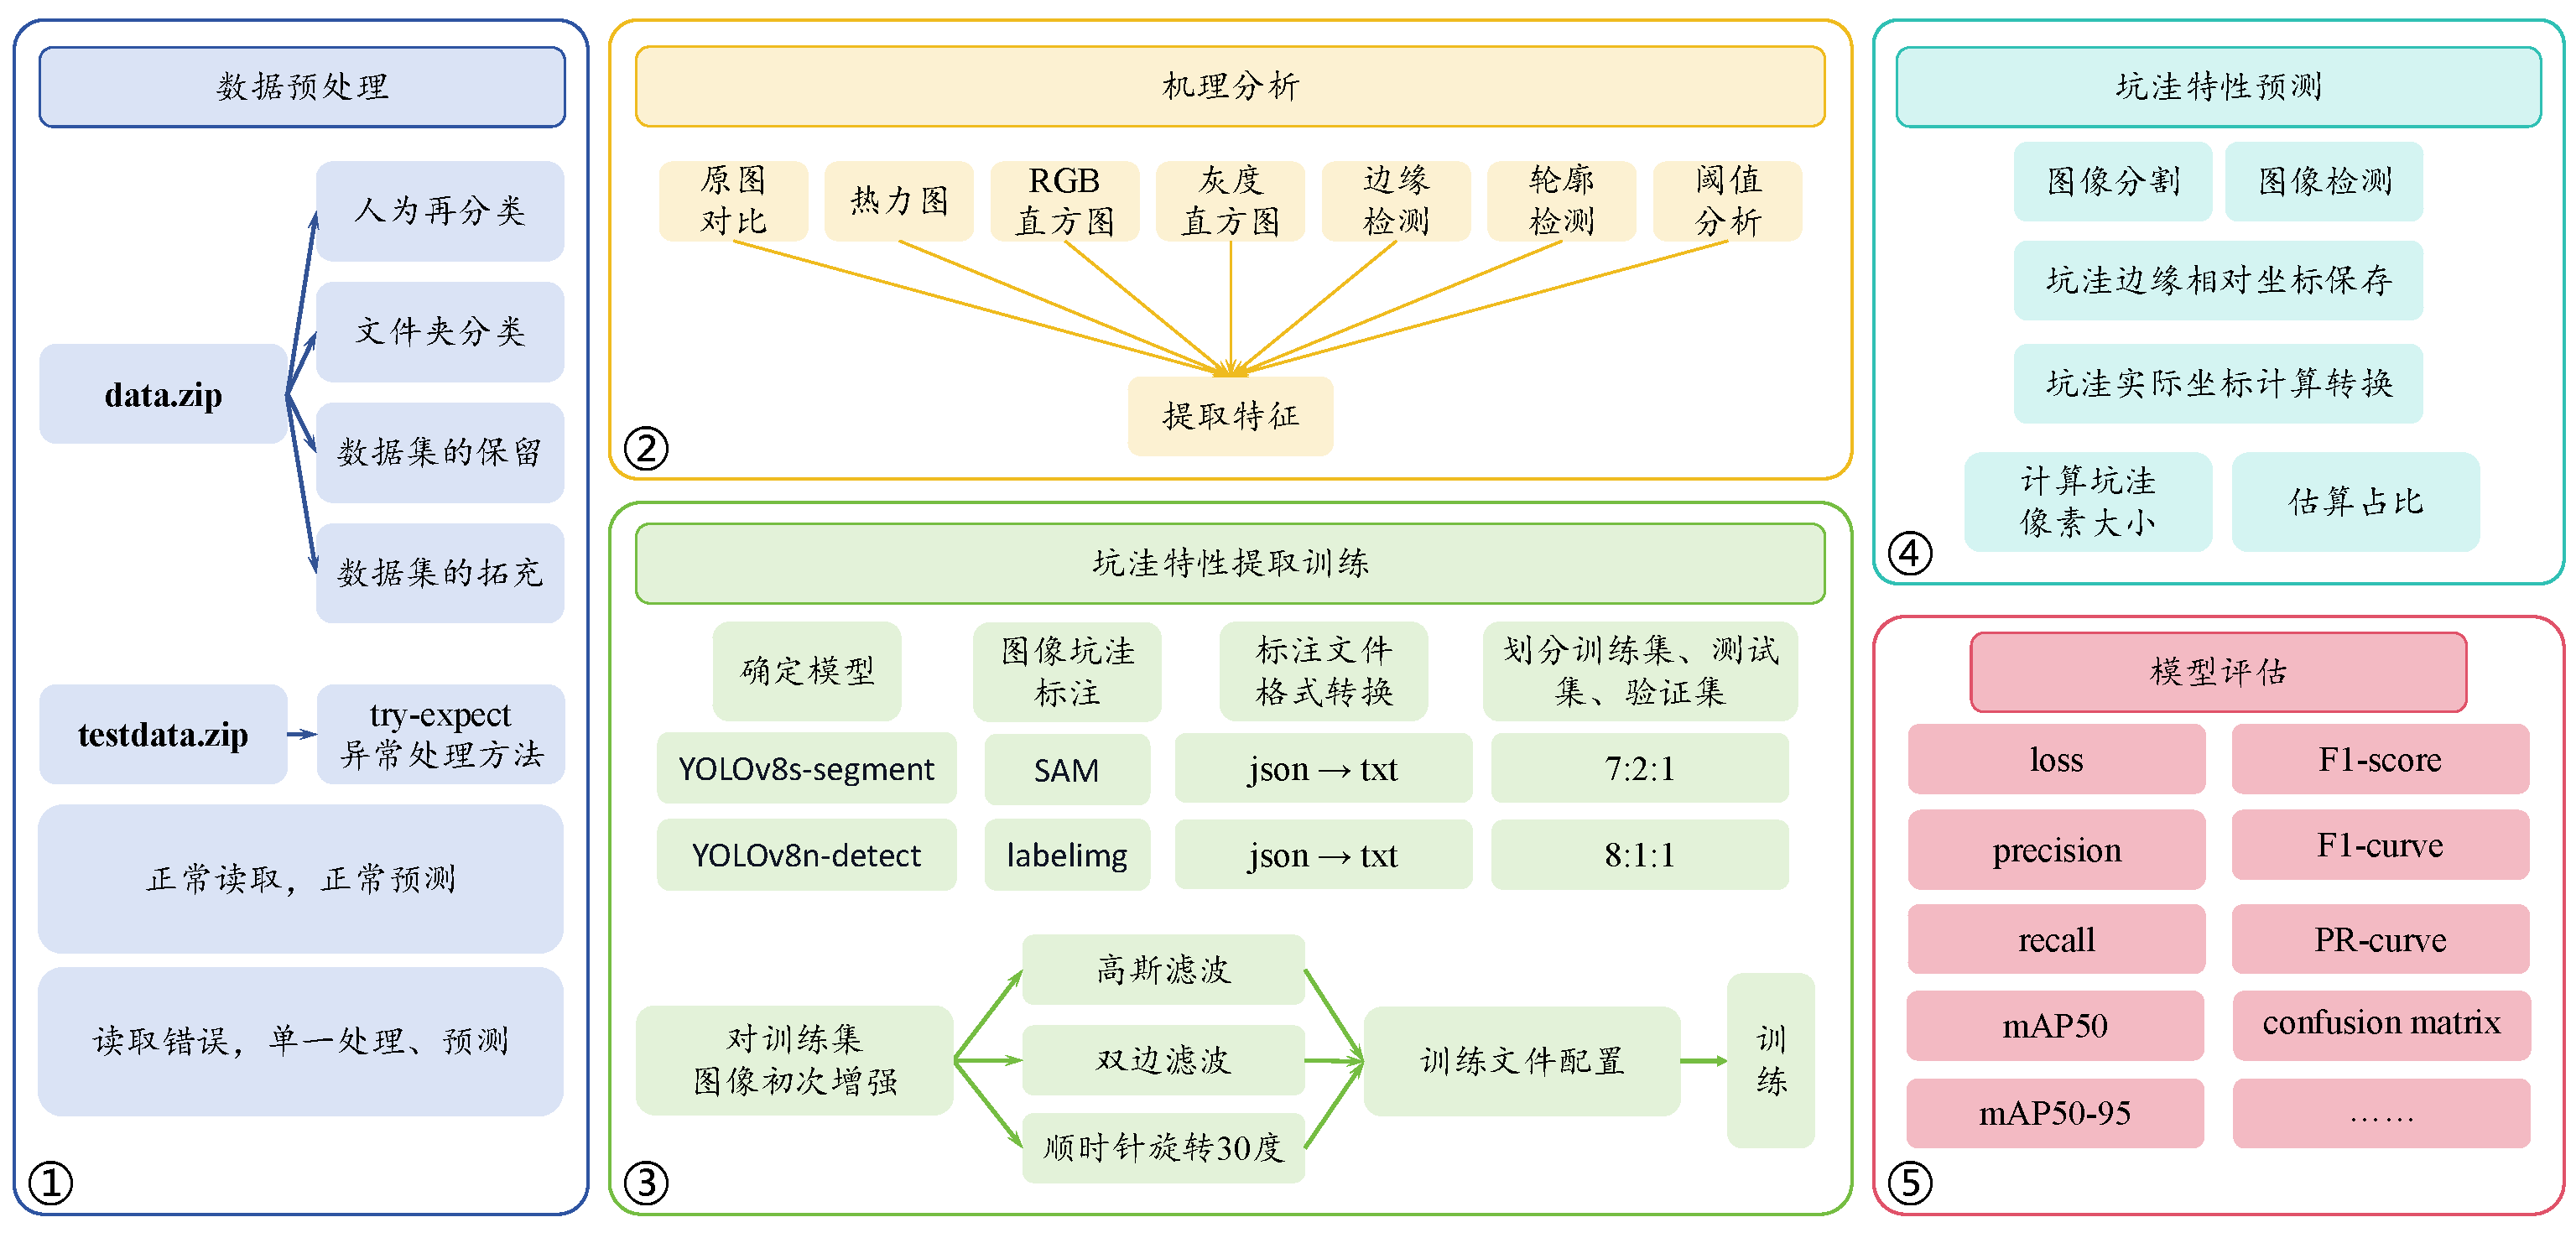
\includegraphics[scale=0.34]{流程图-复赛.pdf}
		\caption{流程图}
		\label{fig:流程图}
	\end{figure}
	\section{模型的假设}
	\begin{itemize}
		\item \textbf{假设一}:所给数据集存在因某些原因而标注异常的图像数据的现象;
		\item \textbf{假设二}:所给数据集未能完整地表现出分类的特征。
	\end{itemize}
	\section{符号说明}
	\begin{center}
		\scalebox{0.9}{
		\begin{tabularx}{0.7\textwidth}{c@{\hspace{1pc}}|@{\hspace{2pc}}X}
			\Xhline{0.08em}
			\textbf{符号} & \multicolumn{1}{c}{\textbf{符号说明}}\\
			\Xhline{0.05em}
			$X$ & 图像横轴像素点的像素值\\
			$Y$ & 图像纵轴像素点的像素值\\
			$I_f$ & 滤波后的图像像素值\\
			$I$ & 原始图像像素值\\
			$G_s$ & 归一化权重\\
			$\Omega$ & 滤波邻域窗口\\
			$F_s$ & 空间域核函数\\
			$F_f$ & 像素值域核函数\\
			$E\left(x\right)$ & 数据均值\\
			$\lambda_n$ & 协方差矩阵特征值\\
			$\boldsymbol{u}$ & 协方差矩阵特征向量\\
			$C$ & SVM惩罚系数\\
			$S$ & 池化区域面积\\
			$N_{\text{TruePredict}}$ & 预测正确样本数\\
			$N_{\text{Predict}}$ & 预测样本总数\\
			\Xhline{0.08em}
		\end{tabularx}}
	\end{center}

	\textbf{注:}这里并未列出其余变量,这是由于它们在不同小节处有不同的含义,这些符号以及上述符号在使用时仍会在相应位置进行详细说明。

	\section{模型的建立与求解}
	\subsection{初赛研究相关结论、坑洼特征分析}\label{分析}
	在初赛中,为了方便模型的分析、建立与求解,因此需要对图像数据进行机理分析,将标记为正常及坑洼的道路进行比较分析,并提取图像的特征。从以下几个方面进行分析:
	\begin{itemize}
		\item \textbf{原图、热力图对比}:分析坑洼与正常道路的表层区别。
		\item \textbf{RGB、灰度直方图}:分析坑洼与正常道路的图像信息分布。
		\item \textbf{边缘、轮廓检测}:分析坑洼与正常道路的边缘、轮廓特征。
		\item \textbf{阈值分割}:分析坑洼与正常道路的阈值分割特征。
	\end{itemize}
	
	但由于图片较多,故我们选择“normal133.jpg”及“potholes1.jpg”进行对比分析。以下是具体分析内容,该部分具体处理代码见\textbf{附录-C.1,Comparative Analysis of Normal and Potholes [正常与坑洼道路的比较分析]}。
	\subsubsection{原图、热力图对比}
	“normal133.jpg”及“potholes1.jpg”原图及热力图对比,如\textcolor{blue}{\cref{fig:原图对比}}及\textcolor{blue}{\cref{fig:热力图对比}}所示\textcolor{blue}{\footnote{本文所有图示、表格均已交叉引用,读者阅读PDF时可点击对应图表,进行跳转。}}。
	\begin{figure}[H]
		\centering
			\centering
			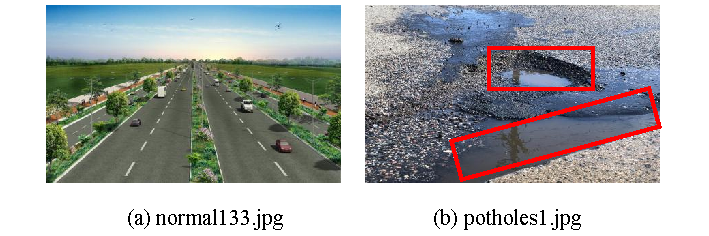
\includegraphics[scale=0.96]{[原图对比]normal133与potholes1.pdf}
			\caption{原图对比}
			\label{fig:原图对比}
	\end{figure}
	
	对比正常道路和坑洼道路的热力图,我们发现若整个道路的状况相同,没有坑洼,则那一片区域的热力值近似相同,热力图呈现的颜色相仿;若道路中的某一块状况与周围不同,如出现坑洼,则出现坑洼的区域热力值发生变化,使在热力图中呈现的颜色与周围存在差异。正常道路热力值基本一致,其热力图呈现色彩差别小,而坑洼道路中非坑洼处与坑洼处热力值相差较大,坑洼处与非坑洼处颜色相比存在较大差异。
	\begin{figure}[H]
		\centering
		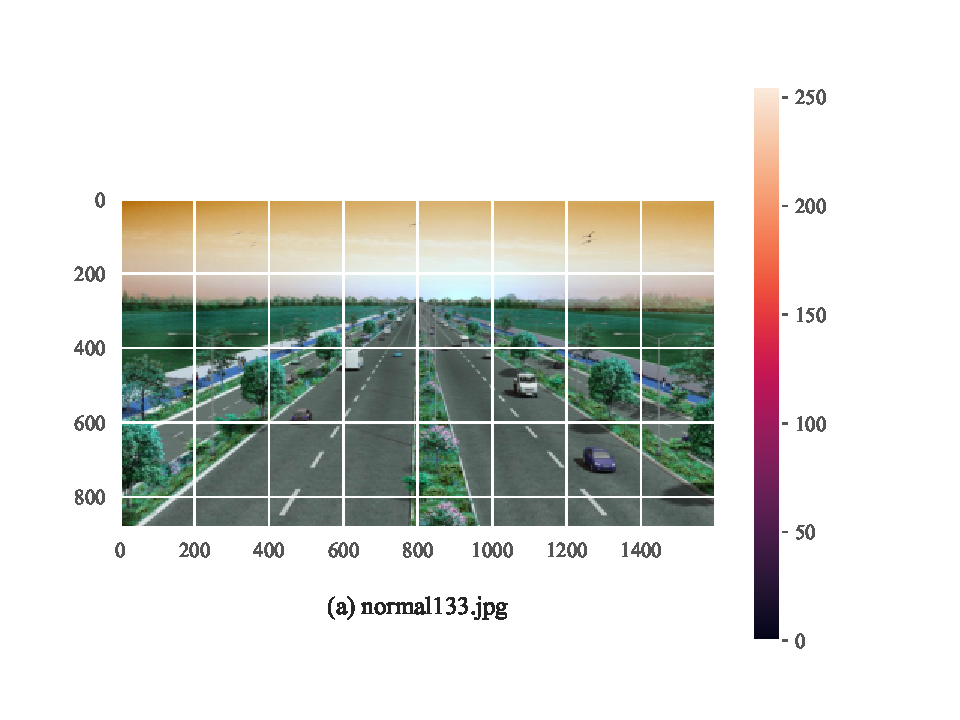
\includegraphics[scale=0.5]{normal133热力图.pdf}
		\hspace{0.3in}
		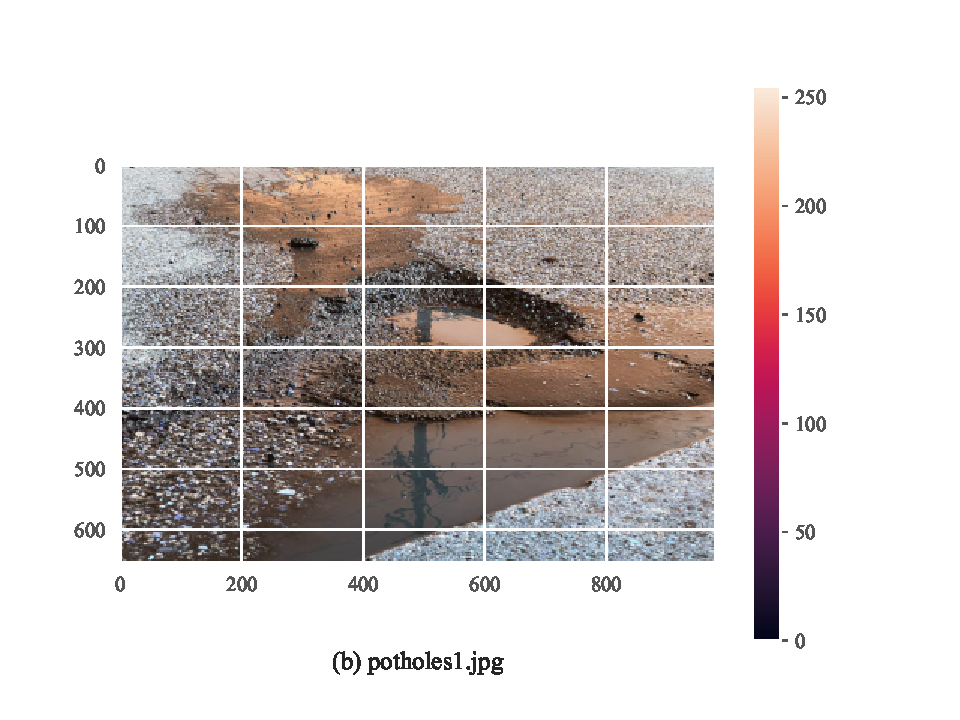
\includegraphics[scale=0.5]{potholes1热力图.pdf}
		\caption{热力图对比}
		\label{fig:热力图对比}
	\end{figure}

	\subsubsection{RGB、灰度直方图}
	“normal133.jpg”及“potholes1.jpg”RGB及灰度直方图对比,如\textcolor{blue}{\cref{fig:RGB对比}}及\textcolor{blue}{\cref{fig:灰度对比}}所示。
	
	观察RGB直方图的对比,我们可以发现两者RGB三色整体变化具有一致性,但正常道路的RGB数值整体高于坑洼道路,且正常道路RGB峰值出现在像素值为$50\text{\textasciitilde}100$之间,而坑洼道路的RGB峰值出现在像素值为$0$与$250$处。

	观察灰度直方图的对比,我们可先发现灰度直方图中正常道路所呈现的峰值远高于坑洼道路,其中坑洼道路的峰值出现在图像两侧,而正常道路的峰值出现在图像的中心位置。此外正常道路数值波动明显大于坑洼道路。故我们认为灰度直方图所展现的数值大小、分布及波动情况可以较好体现道路的坑洼情况。
	\begin{figure}[H]
		\centering
		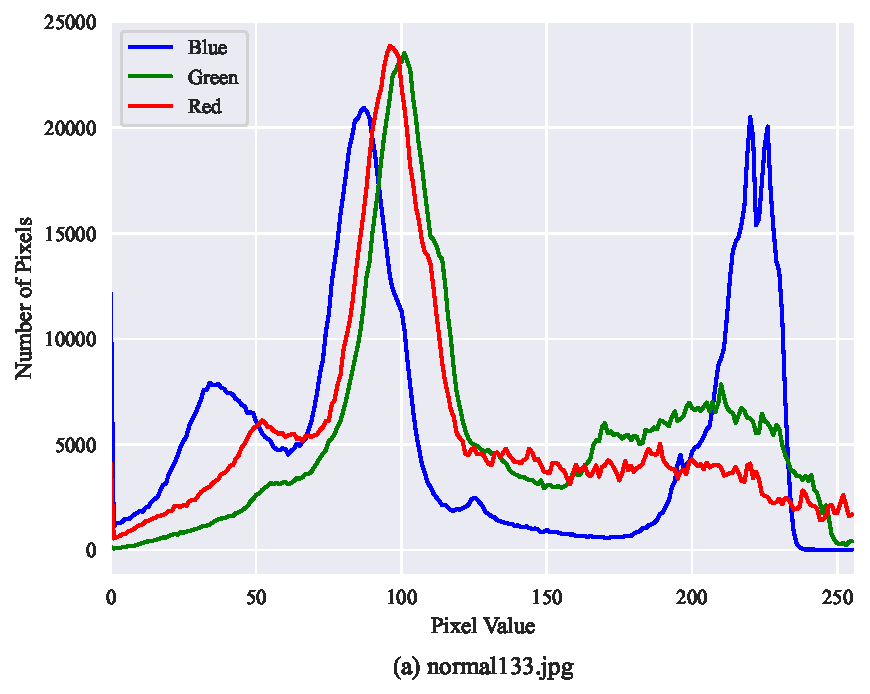
\includegraphics[scale=0.5]{normal133RGB直方图.pdf}
		\hspace{0.3in}
		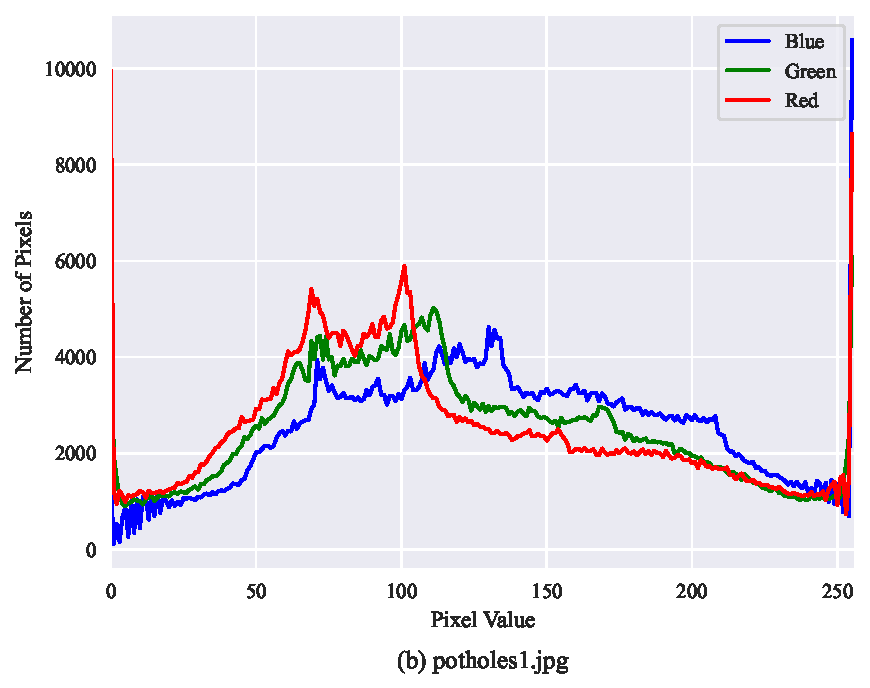
\includegraphics[scale=0.5]{potholes1RGB直方图.pdf}
		\caption{RGB直方图对比}
		\label{fig:RGB对比}
	\end{figure}
	\begin{figure}[H]
		\centering
		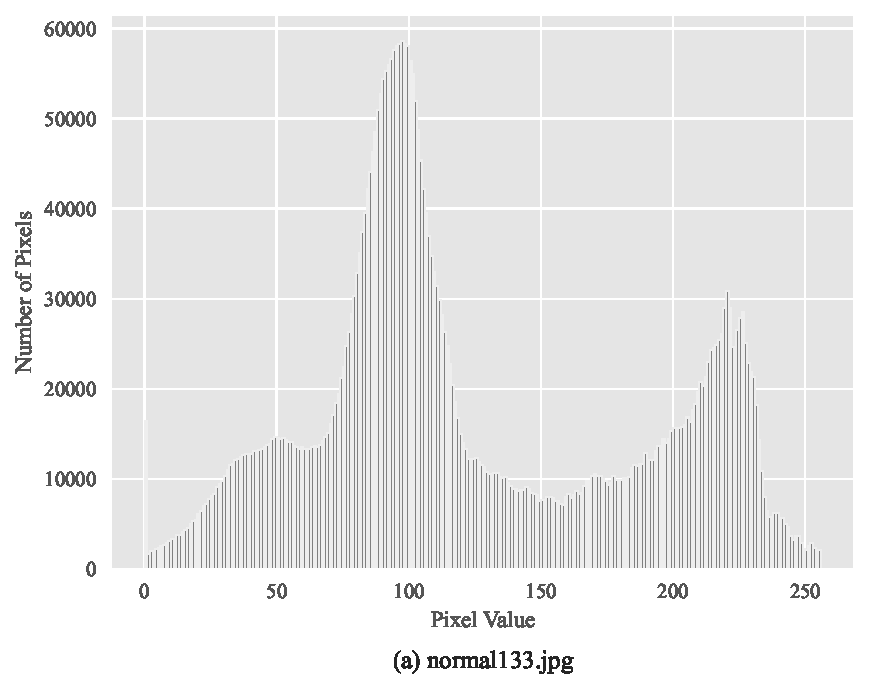
\includegraphics[scale=0.5]{normal133灰度直方图.pdf}
		\hspace{0.3in}
		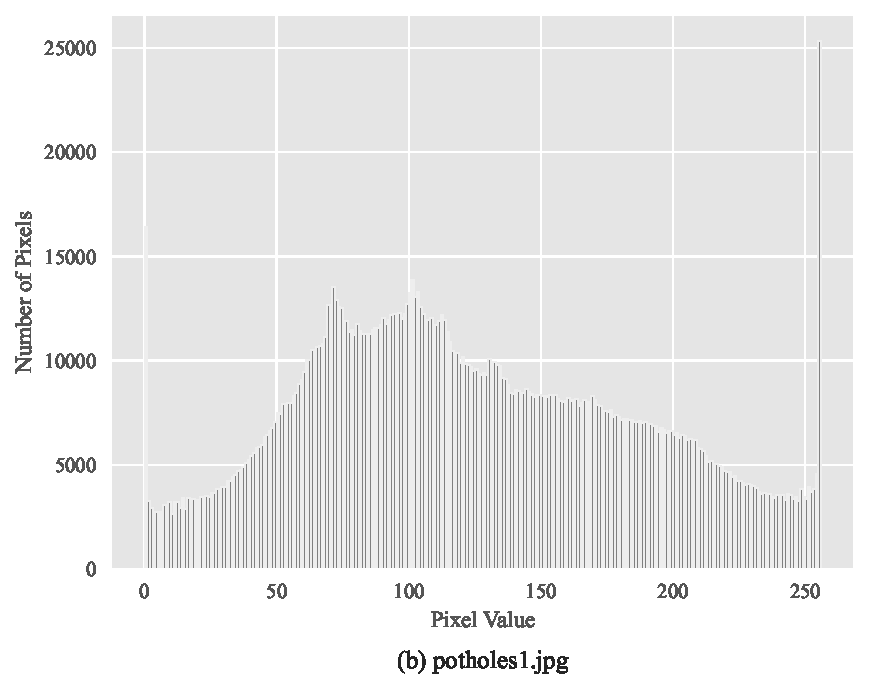
\includegraphics[scale=0.5]{potholes1灰度直方图.pdf}
		\caption{灰度直方图对比}
		\label{fig:灰度对比}
	\end{figure}
	
	\subsubsection{边缘、轮廓检测}
	“normal133.jpg”及“potholes1.jpg”边缘、轮廓检测对比,如\textcolor{blue}{\cref{fig:边缘检测}}及\textcolor{blue}{\cref{fig:轮廓检测}}所示。
	\begin{figure}[H]
		\centering
		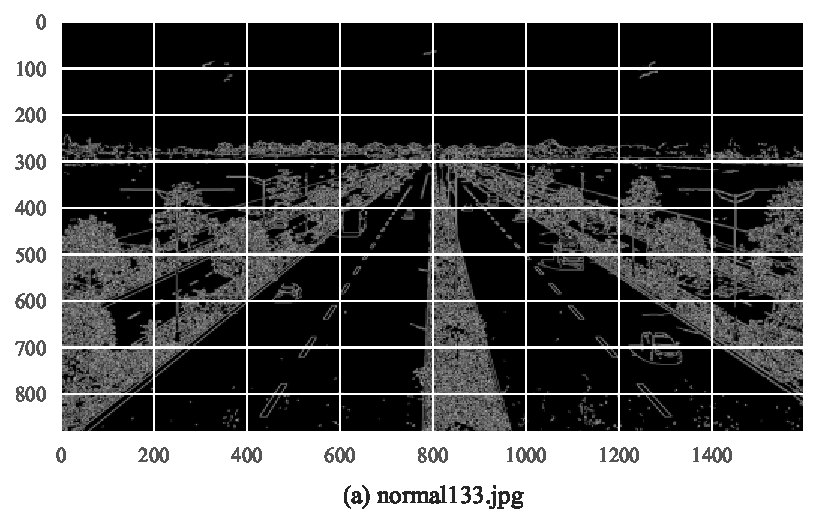
\includegraphics[scale=0.5]{normal133边缘检测.pdf}
		\hspace{0.3in}
		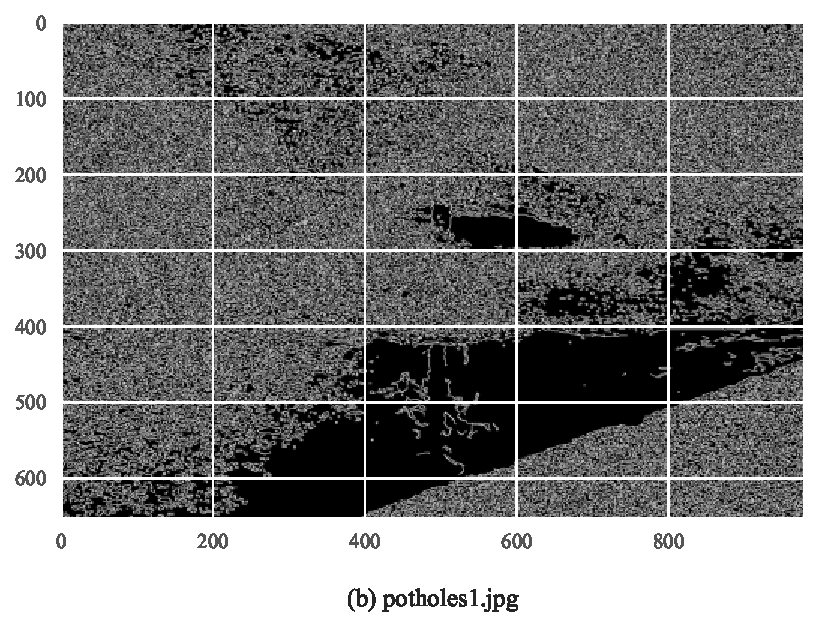
\includegraphics[scale=0.45]{potholes1边缘检测.pdf}
		\caption{边缘检测}
		\label{fig:边缘检测}
	\end{figure}
	观察边缘检测的对比,我们可以发现边缘检测后正常道路色彩连续完整,而坑洼道路的坑洼部分在边缘检测后整体呈现深度黑色,与平整的砂石路面形成了强烈对比。故我们认为采用边缘检测可以较好判断道路状况。

	对道路的图片进行轮廓检测后,我们可以发现检测后无坑洼道路的图片颜色相同,而对于坑洼道路,图片上有很明显的颜色差别。经过分析,我们认为不同的颜色代表了道路的平整与坑洼,进行轮廓检测后,可以通过道路颜色的异同判断道路是否坑洼。
	\begin{figure}[H]
		\centering
		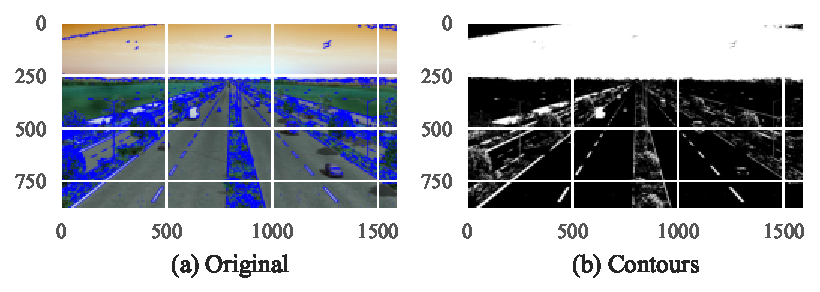
\includegraphics[scale=0.58]{normal133轮廓检测.pdf}
		\hspace{0.3in}
		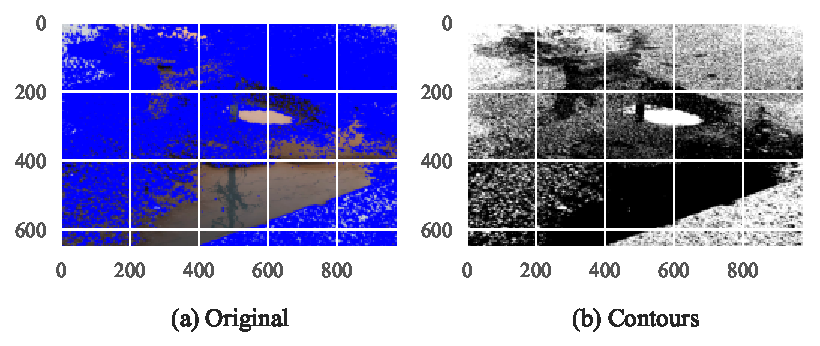
\includegraphics[scale=0.5]{potholes1轮廓检测.pdf}
		\caption{轮廓检测}
		\label{fig:轮廓检测}
	\end{figure}

	\subsubsection{阈值分割}
	“normal133.jpg”及“potholes1.jpg”阈值分割对比,如\textcolor{blue}{\cref{fig:阈值分割}}所示。
	\begin{figure}[H]
		\centering
		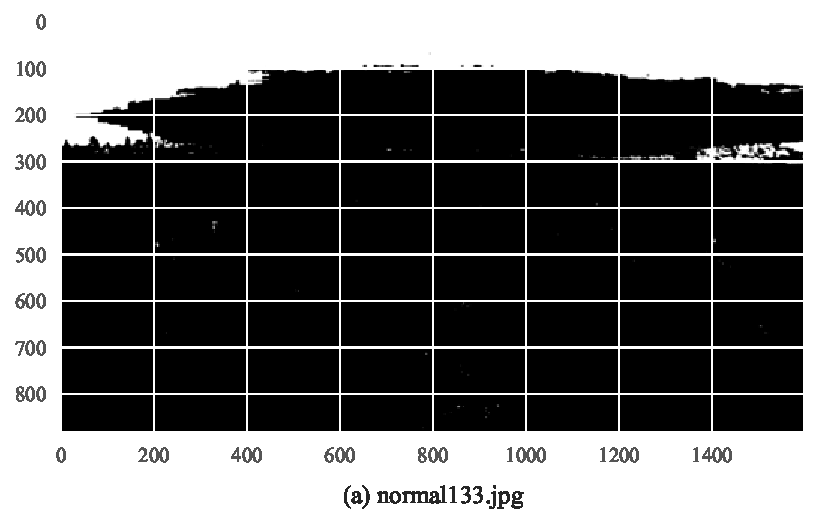
\includegraphics[scale=0.5]{normal133阈值分割.pdf}
		\hspace{0.3in}
		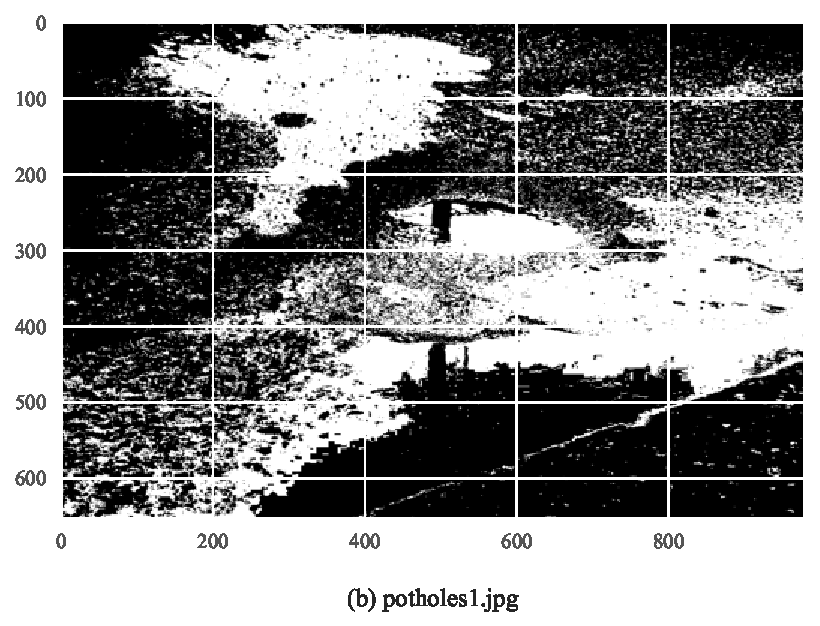
\includegraphics[scale=0.42]{potholes1阈值分割.pdf}
		\caption{阈值分割}
		\label{fig:阈值分割}
	\end{figure}
	阈值分割将图片分为两类区域,对比正常道路与坑洼道路的阈值分割图,正常道路由于整个道路的状态相同,因此经阈值分割后,全部被划分为同一类,故颜色相同;而对于坑洼道路,道路中出现了与周围状态不同的区域,经过阈值分割后,呈现出不同的颜色,黑色为正常的道路,白色为道路中存在的坑洼,色彩对比强烈。

	\subsection{图像文件预处理}\label{图像文件预处理}
	该题原数据集为“data.zip”,包含301张图片,均为“jpg”格式,且在文件名中进行了标注。其中,文件名中包含“normal”字符的表示正常道路,共266张,包含“potholes”字符的为坑洼道路,共35张。考虑到数据的标注严谨性,首先对其进行人为再分类,将标注异常的进行重新标注或剔除。此外,为方便后续模型的分析、建立与求解,我们将“normal”与“potholes”图像文件置于“DATA”文件下的“normal”及“potholes”文件夹中。

	考虑到图像文件较少,用于训练的特征不足,因此对原数据集进行拓充,方法为从网络上获取坑洼道路的图像。

	此外,还需要预先读取测试集图像,以防破损文件影响预测过程。
	\subsubsection{人为再分类}
	考虑到数据的标注严谨性,我们首先对其进行人为再分类,将标注异常的进行重新标注或剔除。对于所给数据集,我们筛选出了以下几张图片,其标注存在问题,需要进行重新标注或剔除,如\textcolor{blue}{\cref{fig:异常图片}}所示,图中所标注的为该图像的原始文件名。
	\begin{figure}[H]
		\centering
		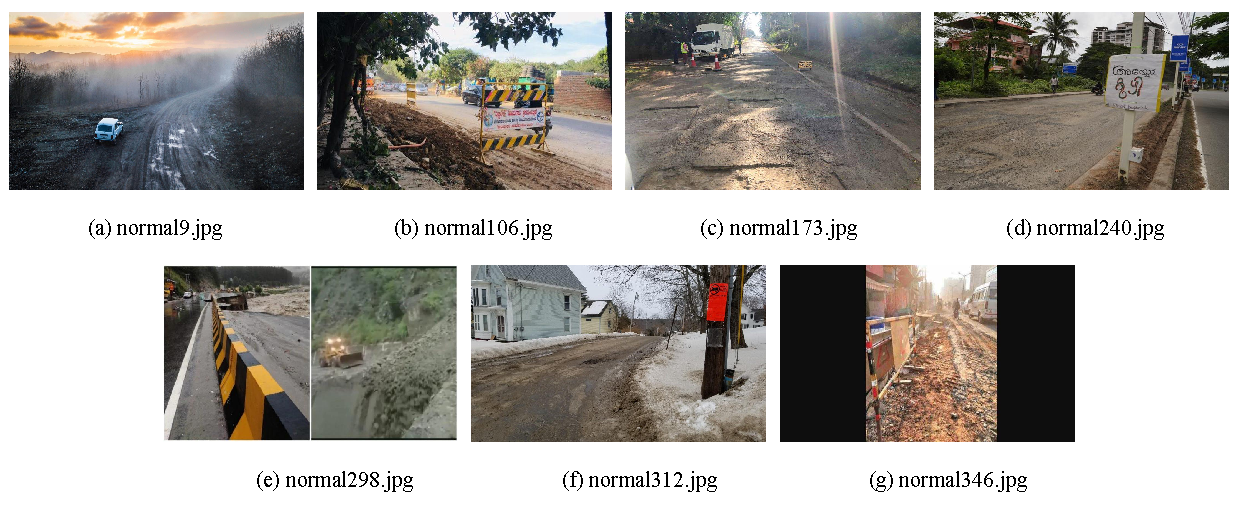
\includegraphics[scale=0.8]{异常图片.pdf}
		\caption{标注异常图片}
		\label{fig:异常图片}
	\end{figure}

	对于上述“(e) normal298.jpg”文件,我们选择剔除,其余划分为“potholes”类。具体处理见\textcolor{blue}{\cref{tab:异常图片处理}}。表中“potholes”代表将该问价视为坑洼道路,而“删除”代表将该文件删除,不参与后续模型的分析、建立、训练等。

\begin{table}[H]
	\centering
	\caption{异常标注图片的处理}
	\scalebox{0.9}{
	  \begin{tabular}{ccc}
	  \toprule
	  \textbf{编号}    & \textbf{原文件名}  & \textbf{处理方式} \\
	  \midrule
	  a     & normal9.jpg & potholes \\
	  b     & normal106.jpg & potholes \\
	  c     & normal173.jpg & potholes \\
	  d     & normal240.jpg & potholes \\
	  e     & normal298.jpg & 删除 \\
	  f     & normal312.jpg & potholes \\
	  g     & normal346.jpg & potholes \\
	  \bottomrule
	  \end{tabular}}
	\label{tab:异常图片处理}
\end{table}

  
	\subsubsection{文件夹分类}
	为了后续模型的分析、建立与求解,我们将“normal”与“potholes”图像文件置于“DATA”文件下的“normal”及“potholes”文件夹中,作为二分类的数据集。该处理我们使用Python的os及shutil库进行处理,首先指定根目录为“DATA”,再在其下创建“normal”与“potholes”文件夹,之后读取“DATA”文件夹下的所有文件,若文件名中含有“normal”字符,则将其放置于“normal”文件夹中,否则放置于“potholes”文件夹中。具体处理代码见\textbf{附录-C.2,Data Preprocessing [数据预处理]}。这里,我们可以大致观测数据集图像,如\textcolor{blue}{\cref{fig:图像数据观测}}所示。
	\begin{figure}[H]
		\centering
		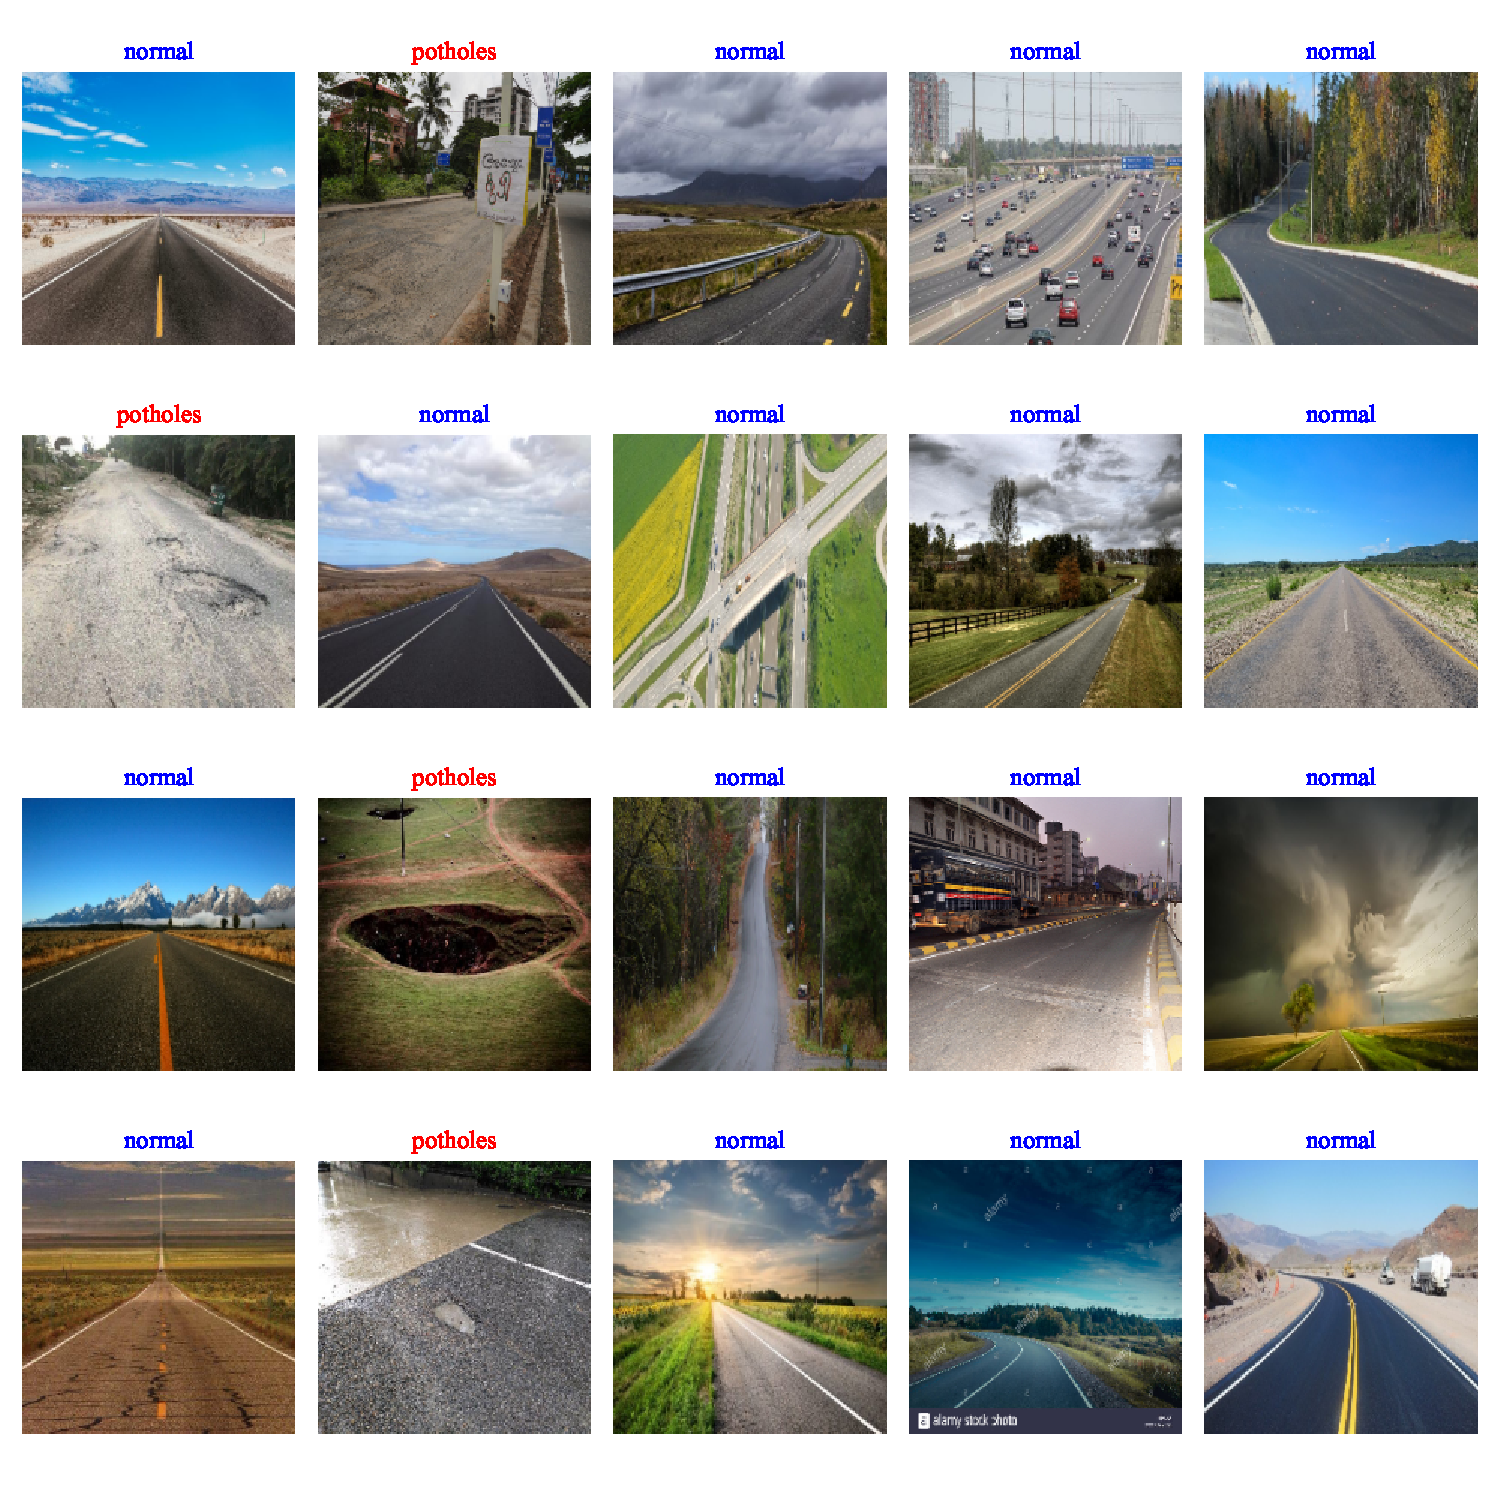
\includegraphics[scale=0.5]{图像数据观测.pdf}
		\caption{图像数据观测}
		\label{fig:图像数据观测}
	\end{figure}
	至此,我们已将所有数据进行了人为再分类,并将数据集分别放于“normal”及“potholes”文件夹中,方便后续的处理。
	
	\subsubsection{原数据集的保留与拓充}
	由于在复赛中,本题任务需要重点分析坑洼道路的特性,因此,这里舍弃“normal”类图像,保留“potholes”图像,共计41张。

	考虑到保留的图像文件较少,学习特征不足,将会影响模型精度。同时,为了加强我们分析的可信度,我们从以下网站收集了坑洼图像,对“potholes”类图像数据进行拓充,来源见\textcolor{blue}{\cref{tab:数据来源}}所示。\textcolor{blue}{\footnote{\textbf{注:}拓充的图为原数据集中尚未出现过的图像,即原数据集为新数据集的子集。}}
	\begin{table}[htbp]
		\centering
		\caption{拓充数据来源}
		\scalebox{0.9}{
		  \begin{tabular}{cc}
		  \toprule
		  \textbf{数据源} & \textbf{网址} \\
		  \midrule
		  Kaggle & \url{https://www.kaggle.com/} \\
		  Github & \url{https://github.com/} \\
		  百度图片  & \url{https://image.baidu.com/} \\
		  \bottomrule
		  \end{tabular}}
		\label{tab:数据来源}
	  \end{table}
	\subsubsection{测试集数据预读取}\label{预读取}
	此外,还需要预先读取测试集图像,以防破损文件影响预测过程。这里我们使用try-except异常处理方法,测试文件是否能够正常读取,方便后续进行预测。
	
	经过测试,发现存在一个文件读取失败,为“guy7iodk.jpg”。因此,对于该张图片,我们对其进行人为处理,再重新读取。具体方法见\textcolor{blue}{\nameref{预测}}。
	
	\subsection{YOLOv8模型简述}

	YOLOv8是Ultralytics公司于2023年1月10日开源的YOLOv5的下一个重大更新版本,目前支持图像分类、物体检测、实例分割、目标追踪、姿态估计任务\textcolor{blue}{\cite{YOLO任务}}。

	YOLOv8是一个SOTA模型,其建立在曾经的版本的基础上引入新的功能,并进行一定改进,从而进一步提升性能与灵活性。具体创新包\textbf{括骨干网络(Backbone Network)}、\textbf{Anchor-Free检测头(Anchor-Free Detection Head)}和\textbf{损失函数(Loss Function)}\textcolor{blue}{\cite{YOLO架构}},模型结构如\textcolor{blue}{\cref{fig:YOLO架构}}所示\textcolor{blue}{\footnote{该架构图来源于:\url{https://mmyolo.readthedocs.io/en/latest/recommended_topics/algorithm_descriptions/yolov8_description.html},原作者为RangeKing@github,其Github主页:\url{https://github.com/RangeKing}。}}。
	\begin{figure}[H]
		\centering
		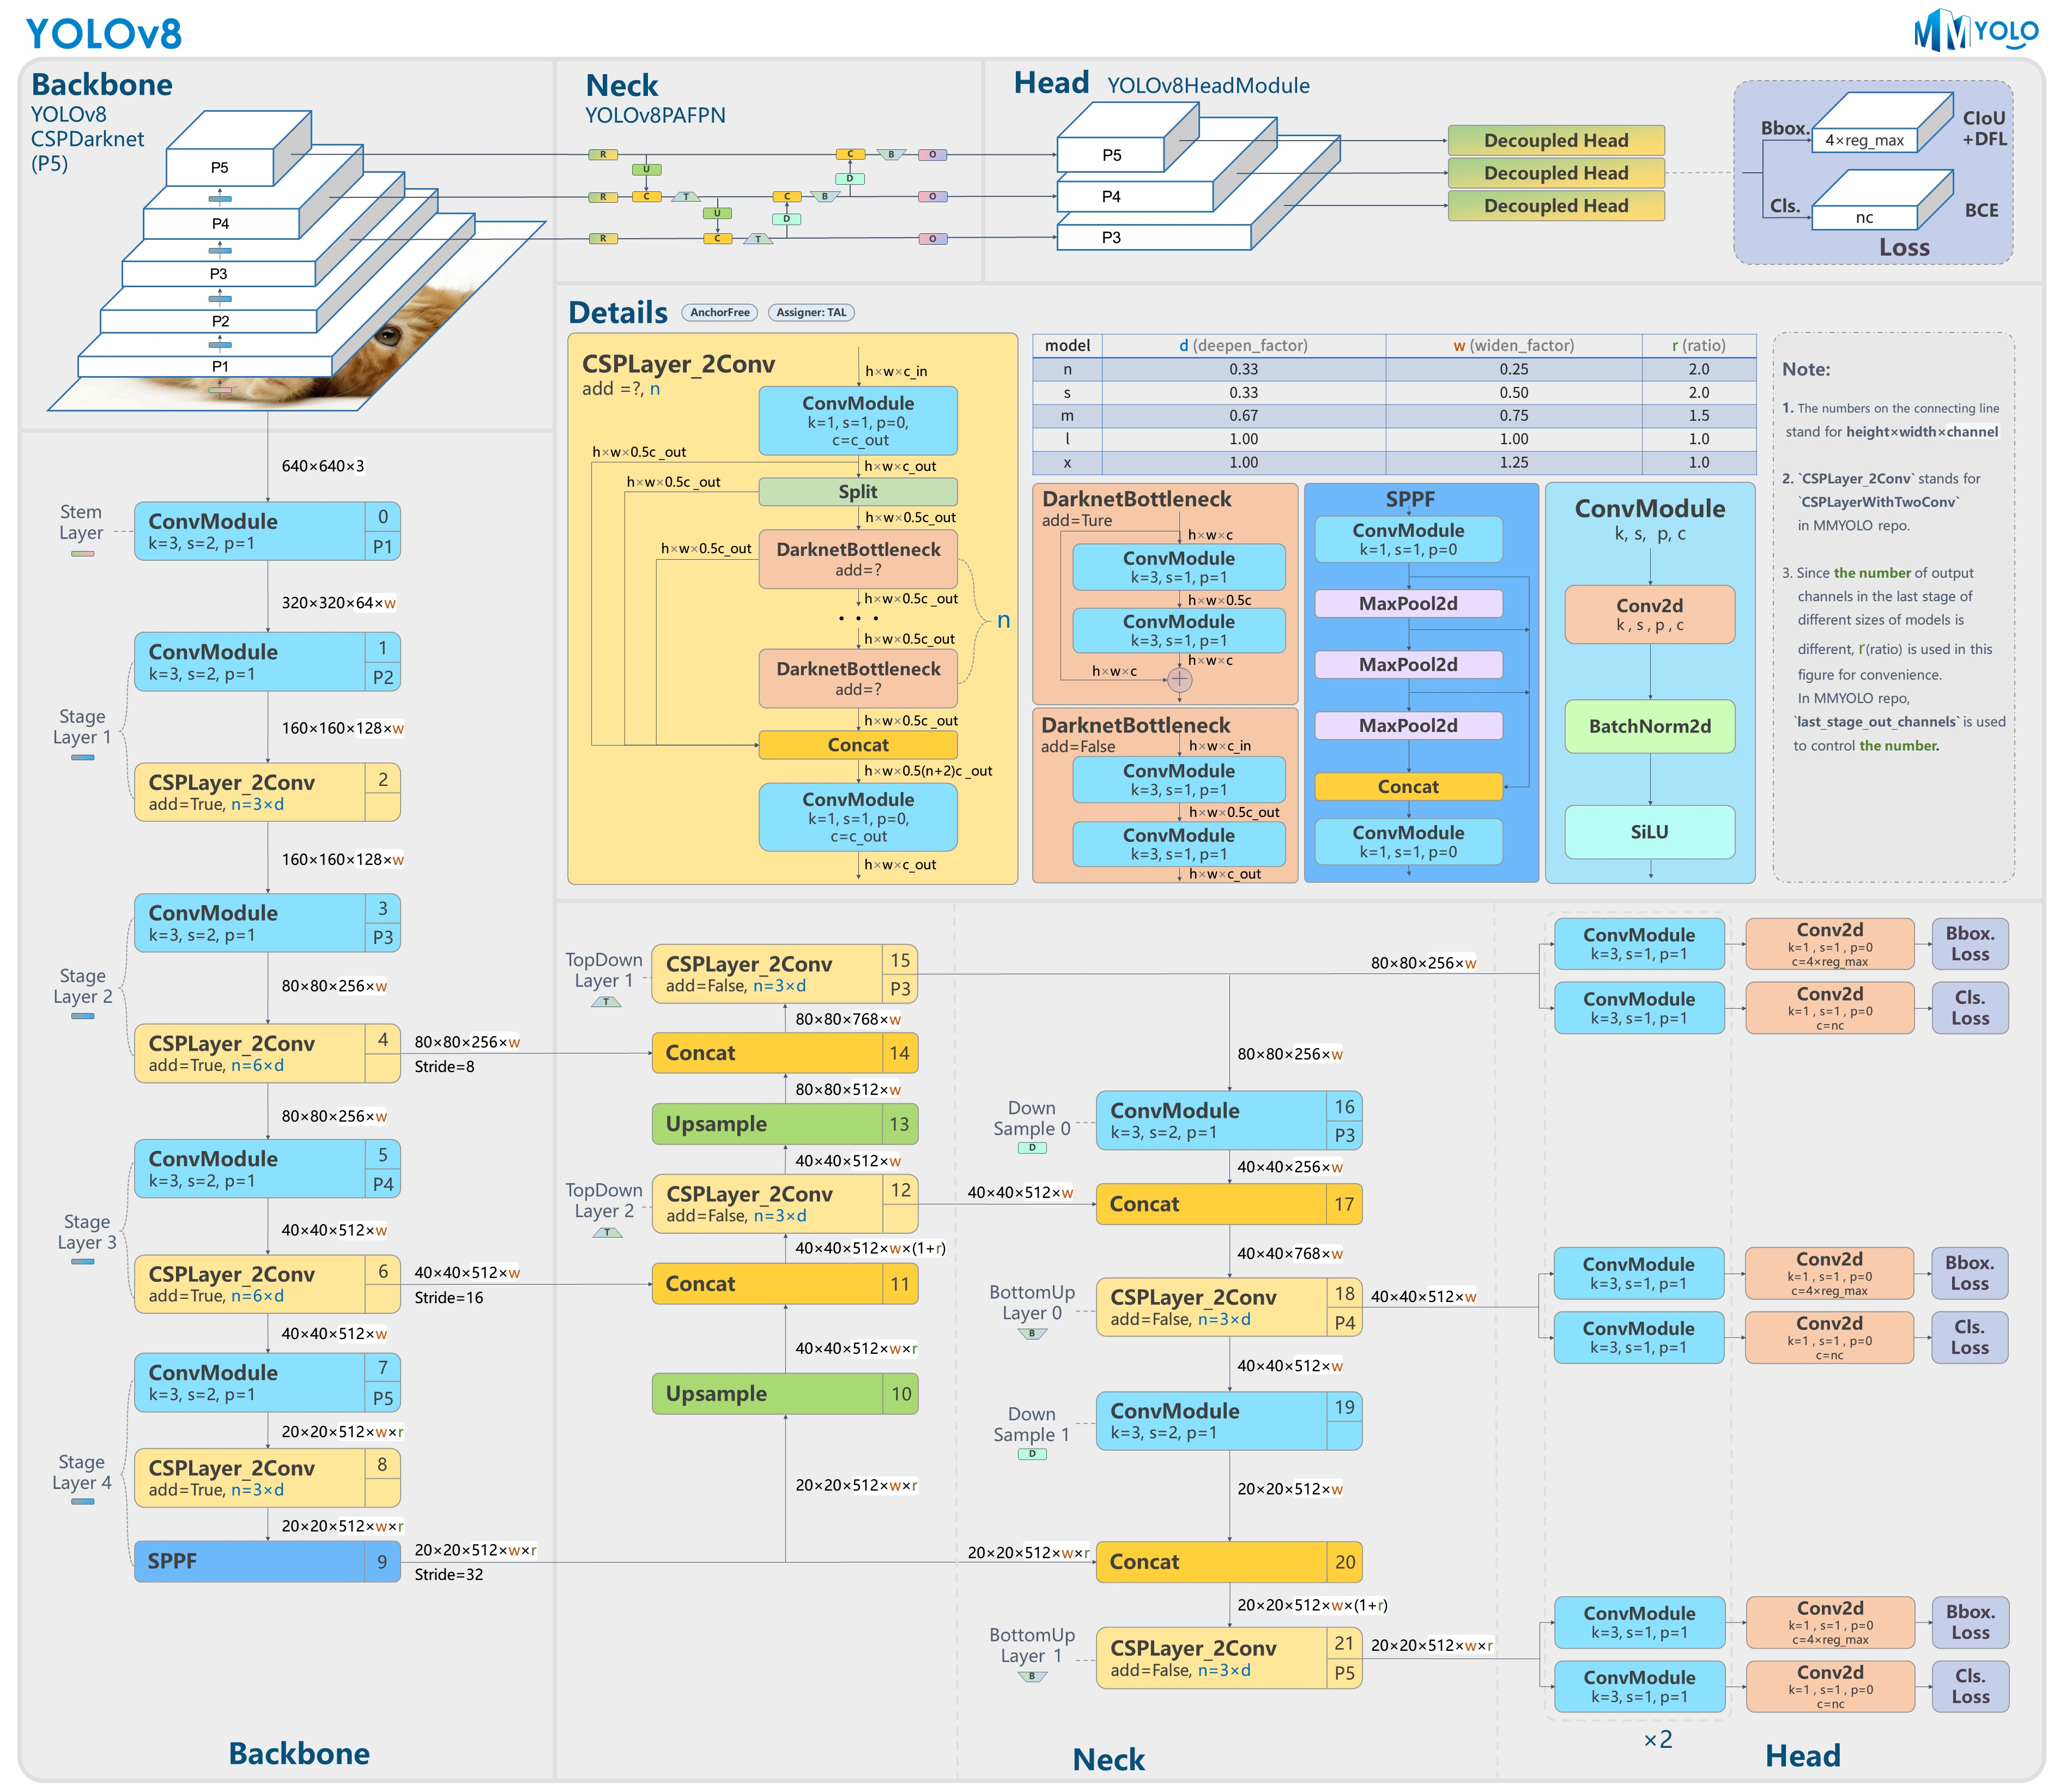
\includegraphics[scale=0.14]{YOLOv8架构}
		\caption{YOLOv8模型架构}
		\label{fig:YOLO架构}
	\end{figure}
	YOLOv8主要可分为Input 输入端、Backbone骨干神经网络、Neck混合特征网络层和Head预测层网络4个部分\textcolor{blue}{\cite{YOLOv8简述}}。
	
	\begin{itemize}
		\item \textbf{Input}:输入端方法包含的功能模块有:\textbf{马赛克(Mosaic)数据增强}、\textbf{自适应锚框(Anchor)计算}、\textbf{自适应图片缩放}和\textbf{Mixup数据增强}\textcolor{blue}{\cite{YOLO数据增强}}。马赛克数据增强通过将4张图像进行随机的缩放、裁剪和打乱分布方式等操作来重新拼接图像,从而丰富检测的数据集。在每次训练数据之前,自适应锚框计算会选择最合适锚框尺寸,自动匹配最佳锚框,并将在目标检测中将两幅图像的像素值按图像透明度的通道信息进行线性融合。
		\item \textbf{Backbone Network}:骨干网络用来提取图像特征,包括\textbf{注意力(Focus)机制模块}、\textbf{跨阶段局部网络(Cross Stage Partial Network, CSP)}和\textbf{空间金字塔池化(Spatial Pyramid Pooling, SPP)结构}四个模块。先将图片进行切片,再将新得到的图片经过卷积操作,生成没有信息丢失的两倍下的采样特征图。
		\item \textbf{Neck}:Neck混合特征网络层由卷积层和C2f组成,通过\textbf{路径聚合网络(Path Aggregation Network, PAN)}和\textbf{特征金字塔网络(Feature Pyramid Network, FPN)}的结构对特征进行多尺度融合,将图像特征传递到预测层。
		\item \textbf{Head}:Head预测层采用\textbf{解耦检测头(Decoupled-Head)}\textcolor{blue}{\cite{Head}},通过不同的分支进行运算,提升检测效果。
	\end{itemize}

	\subsection{坑洼特性提取模型的训练}
	为对坑洼特性进行提取,我们需要建立基于YOLOv8的segment图像分割及YOLOv8的detect图像检测模型,对道路的坑洼特性进行学习、训练。在此之前需要对图像进行标注,标注文件的格式转换,训练集、测试集、验证集三者的划分,对训练集进行数据增强,配置训练文件。待模型训练完成后,再读取迭代过程中最优模型对测试集数据的坑洼边缘进行提取。
	\subsubsection{图像坑洼标注}
	首先,需要对图像中的坑洼位置进行标注,对于本文所建立的两个YOLOv8模型,使用不同的标注方法,标注过程示意图如\textcolor{blue}{\cref{fig:图像坑洼标注}}所示。
	\begin{itemize}
		\item \textbf{YOLOv8s-Segment}:基于Segment Anything Model的交互式半自动图像分割标注工具(Interactive Semi-automatic Annotation Tool for image segmentation with Segment Anything Model, ISAT-SAM);
		\item \textbf{YOLOv8n-Detect}:Labelimg标注。
	\end{itemize}
	\begin{figure}[H]
		\centering
		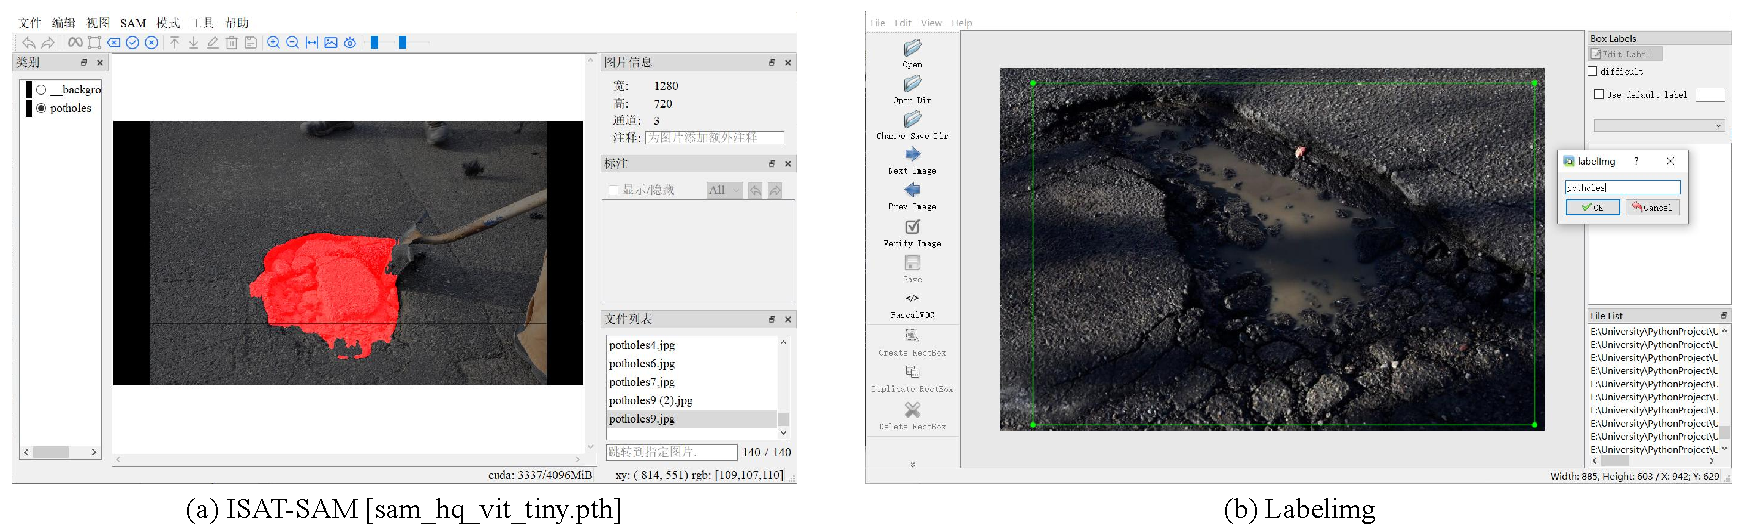
\includegraphics[scale=0.5]{坑洼标注.pdf}
		\caption{图像坑洼标注}
		\label{fig:图像坑洼标注}
	\end{figure}

	两者比较如下:
	\begin{itemize}
		\item \textbf{ISAT-SAM}:ISAT-SAM是一种基于SAM的交互式半自动图像分割标注工具,本文所使用的预训练模型为“sam\_hq\_vit\_tiny.pth”。该工具支持手动标注多边形、连点绘制、标注二次修改、重叠目标调整遮挡关系、标注结果预览、单独线程进行Sam Encoder计算,降低切换图片的卡顿感\textcolor{blue}{\cite{ISAT-SAM}}。同时,其相比于其他人工标注方法,采用SAM,大大提升了标注效率,且边缘处理更精准。标注输出格式为JSON文件。
		\item \textbf{Labelimg}:Labelimg是一个可视化的图像标注工具。其是用Python编写的,并将Qt用于图形界面。批注以PASCAL VOC格式(ImageNet使用的格式)另存为XML文件\textcolor{blue}{\cite{Labelimg}}。其仅可标注矩形,因此多用于图像目标的检测任务。
	\end{itemize}
	\subsubsection{标注文件格式转换}
	由于上述两种标注方法生成的格式分别为JSON文件和XML文件,而YOLOv8模型所需的标注文件格式为TXT文件,因此需要对其进行格式转换。这里我们使用Python进行处理,具体处理代码见\textbf{附录-C.4,isat2txt [ista转txt]}及\textbf{附录-C.5 xml2txt [xml转txt]}。

	这里我们以“potholes22.jpg”为例,原图见\textcolor{blue}{\cref{fig:potholes22}};两种标注方法转换前与转换后的对比如\textcolor{blue}{\cref{fig:格式转换}}所示。
	\begin{figure}[H]
		\centering
		\begin{minipage}{0.45\linewidth}
		  \centering
		  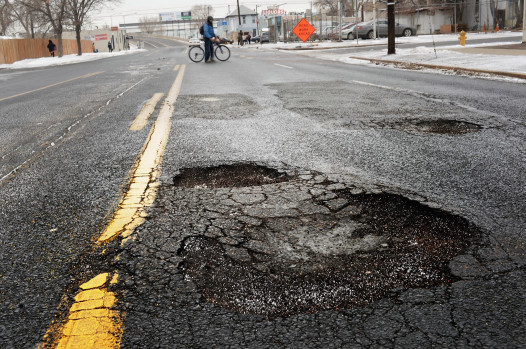
\includegraphics[width=0.7\linewidth]{potholes22}
		  \caption{“potholes22.jpg”原图}
		  \label{fig:potholes22}
		\end{minipage}
		%qquad
		\begin{minipage}{0.45\linewidth}
		  \centering
		  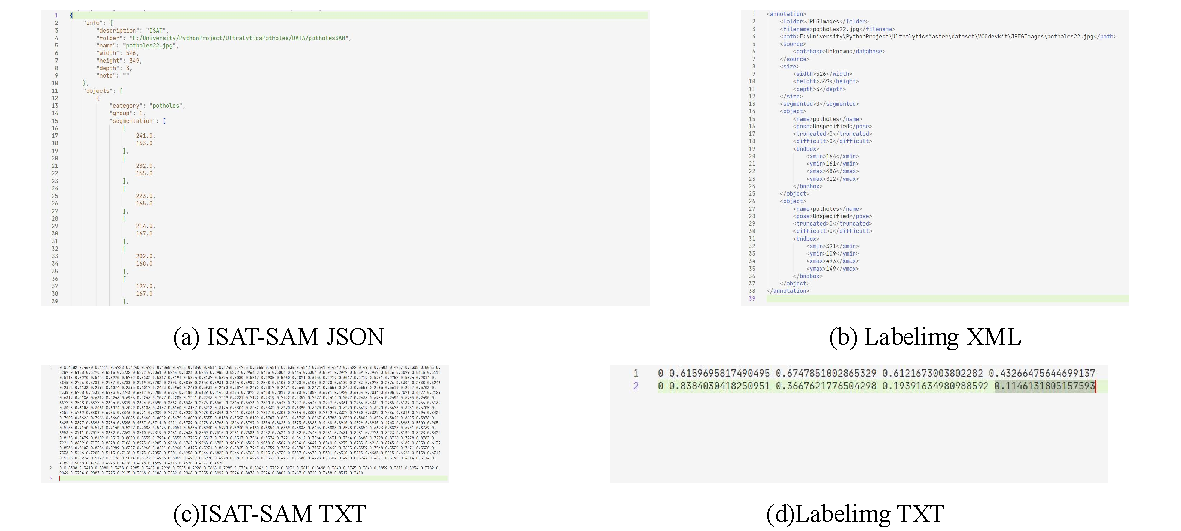
\includegraphics[width=1.0\linewidth]{格式转换.pdf}
		  \caption{格式转换前后文件}
		  \label{fig:格式转换}
		\end{minipage}
	\end{figure}

	\subsubsection{划分训练集、测试集、验证集}
	对于模型的学习,我们需要对数据集进行划分,划分为训练集、测试集以及验证集。
	\begin{itemize}
		\item \textbf{训练集}:用于模型的训练;
		\item \textbf{测试集}:用于对模型性能的评估分析,检验模型效果;
		\item \textbf{验证集}:用于在训练阶段验证模型训练效果,选择超参数。
	\end{itemize}
	
	对于本文所建立的两个YOLOv8模型,我们设置训练集、测试集、验证集的比例见\textcolor{blue}{\cref{tab:比例设置}}。

\begin{table}[H]
	\centering
	\caption{模型训练集、测试集、验证集的划分比例}
	\scalebox{0.9}{
	  \begin{tabular}{cccc}
	  \toprule
	  \textbf{模型名称} & \textbf{训练集} & \textbf{测试集} & \textbf{验证集} \\
	  \midrule
	  YOLOv8n-Detect & 8     & 1     & 1 \\
	  YOLOv8n-Segment & 7     & 2     & 1 \\
	  \bottomrule
	  \end{tabular}}
	\label{tab:比例设置}
  \end{table}
  	具体实现代码见\textbf{附录-C.6,Segment Spilt Data [图像分割数据集划分]}以及\textbf{附录-C.7,Detect Spilt Data [图像检测数据集划分]}。
	\subsubsection{训练集图像初次增强}
	观察数据集,发现其特征多数存在相似性;同时,数据集样本较少。因此,为避免模型的过拟合与欠拟合,这里我们需要对训练集进行初步的数据增强\textcolor{blue}{\footnote{\textbf{注意:}这里数据增强是在划分训练集与测试集之后的,并且仅对训练集数据进行增强,并不对测试集进行划分。这是由于,若在划分训练集与测试集之前进行增强,则会造成数据泄露,影响模型的准确性,以及对未知数据的泛化能力。}}。从而增强模型对于未知数据集的泛化能力,提升模型的稳健性。

	这里,我们选用线性滤波中的\textbf{高斯滤波(Gauss Blur)}、非线性滤波中的\textbf{双边滤波(Bilateral Blur)}、以及对图像进行\textbf{顺时针旋转$\boldsymbol{\frac{\pi}{6}}$}处理。
	\begin{itemize}
		\item \textbf{高斯滤波}是一种线性平滑滤波。其基本原理是使用高斯核对图像进行卷积操作,进行加权平均的过程。每一个像素点的值,都由其邻域内的其他像素值和本身经过加权平均后得到。高斯核的标准差和大小决定了滤波器的效果,标准差越小,滤波器的效果越不明显,但是不会导致图像的细节信息丢失。其权值随着距离中心像素点的距离增加而逐渐减小,从而保留了图像的边缘信息。使用公式如下:
		\begin{equation}
			G\left(X,Y\right)=\frac{1}{2\pi\sigma^2}\exp\left(-\frac{X^2+Y^2}{2\sigma^2}\right)
		\end{equation}
		\item \textbf{双边滤波}是一种基于高斯滤波的非线性滤波方法,目的是解决高斯滤波造成的边缘模糊。结合图像的空间邻近度和像素值相似度,同时考虑空域信息和灰度相似性,实现保边去噪。双边滤波器比高斯滤波多一个高斯核。它是基于像素颜色分布的高斯滤波函数,所以在边缘附近,当两个像素距离很近时,只有同时当颜色很接近时影响才会较大,反之,虽然距离很近,但颜色差距较大,那么平滑权重也会很小。
		
		为实现双边滤波,我们首先定义滤波器的参数,即空间域核函数和像素值域核函数;然后计算出每个像素在空间域和像素值域上的权重;最后根据计算得到的权重,对每个像素的周围像素进行加权平均,以得到滤波后的像素值。其公式可表示为:
		\begin{equation}
			I_f\left( X,Y \right) =\frac{\sum_{\left( i,j \right) \in \Omega}{I\left( X+i,Y+j \right) \cdot F_s\left( i,j \right)}\cdot F_f\left[ I\left( X,Y \right) ,I\left( X+i,Y+j \right) \right]}{G_s\left( X,Y \right)} 
		\end{equation}
		上式中各参量含义如下:
		\begin{itemize}
			\item $I_f\left(X,Y\right)$:滤波后的图像像素值;
			\item $I\left(X,Y\right)$:原始图像像素值;
			\item $G_s\left(X,Y\right)$:归一化权重;
			\item $\Omega$:滤波邻域窗口;
			\item $F_s\left(i,j\right)$:空间域核函数;
			\item $F_f\left[ I\left( X,Y \right) ,I\left( X+i,Y+j \right) \right]$:像素值域核函数。
		\end{itemize}
	\end{itemize}
	
	这里,我们随机选择一张图片,将其经过上述处理后的图像一一展示,如\textcolor{blue}{\cref{fig:原图高斯双边滤波及旋转对比}}所示。经过上述处理后,在一定程度上可以增加训练集数据的多样性,从而模型可以学习到更多关于正常或坑洼道路的特征,因而有利于提升模型的泛化能力。
	\begin{figure}[H]
		\centering
		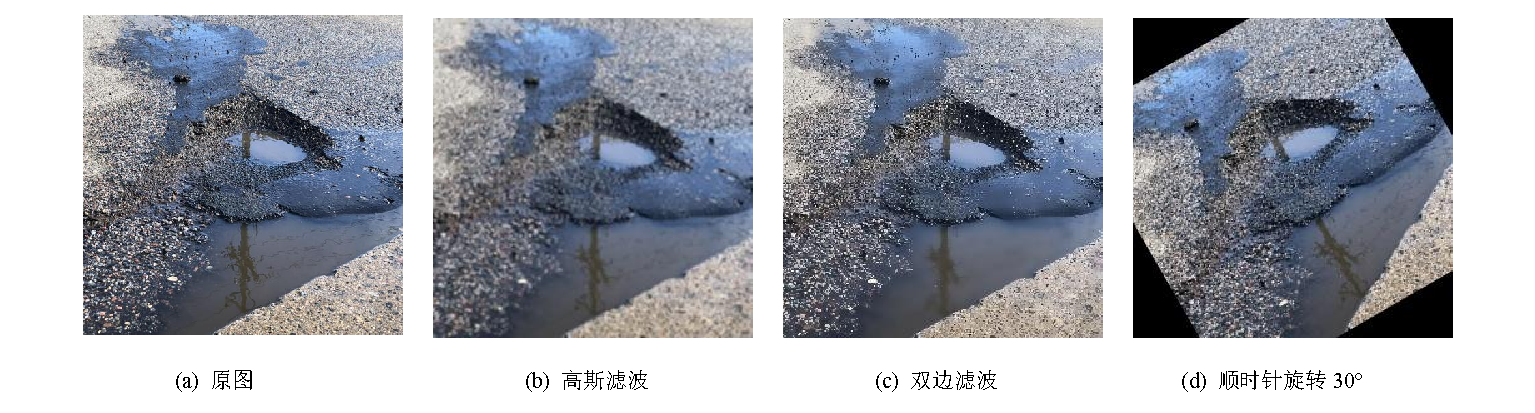
\includegraphics[scale=0.6]{原图高斯双边滤波及旋转对比.pdf}
		\caption{原图、高斯滤波、双边滤波、顺时针旋转30度}
		\label{fig:原图高斯双边滤波及旋转对比}
	\end{figure}

	\subsubsection{训练文件配置}
	至此,我们还需要预训练模型,这里我们选用YOLOv8s-seg及YOLO8n分别作为图像分割及图像检测的基础模型,命名为YOLOv8-Segment及YOLOav8-Detect。此外,我们还需要配置训练文件,主要配置文件见\textcolor{blue}{\cref{tab:配置文件}}。

\begin{table}[htbp]
	\centering
	\caption{模型配置文件}
	\scalebox{0.9}{
	  \begin{tabular}{cc}
	  \toprule
	  \textbf{模型名称} & \textbf{配置文件} \\
	  \midrule
	  YOLOv8-Segment & segment.yaml与yolov8-seg.yaml \\
	  YOLOv8-Detect & detect.yaml \\
	  \bottomrule
	  \end{tabular}}
	\label{tab:配置文件}
  \end{table}
  
	\subsubsection{模型的训练}
	\begin{itemize}
		\item \textbf{YOLOv8s-Segment}

		在训练时,模型会生成数据集的相关特征,如\textcolor{blue}{\cref{fig:YOLOv8s-Segment训练数据集特征}}所示。
		\begin{figure}[H]
			\centering
			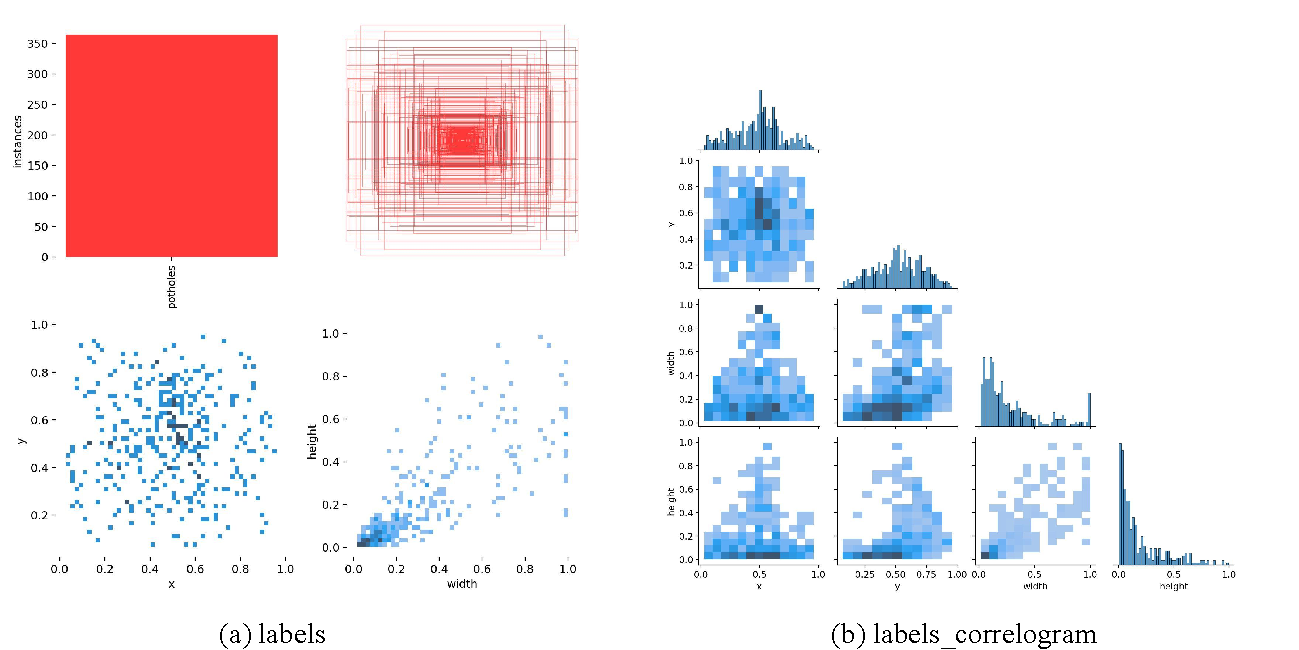
\includegraphics[scale=0.5]{Figures/segment/SegementLabels.pdf}
			\caption{YOLOv8s-Segment训练数据集特征}
			\label{fig:YOLOv8s-Segment训练数据集特征}
		\end{figure}

		同时,YOLOv8模型也会对训练集数据进行增强,有\textbf{马赛克(Mosaic)数据增强}、\textbf{自适应锚框(Anchor)计算}、\textbf{自适应图片缩放}和\textbf{Mixup数据增强},如\textcolor{blue}{\cref{fig:YOLOv8s-Segment训练数据集增强}}所示。
		\begin{figure}[H]
			\centering
			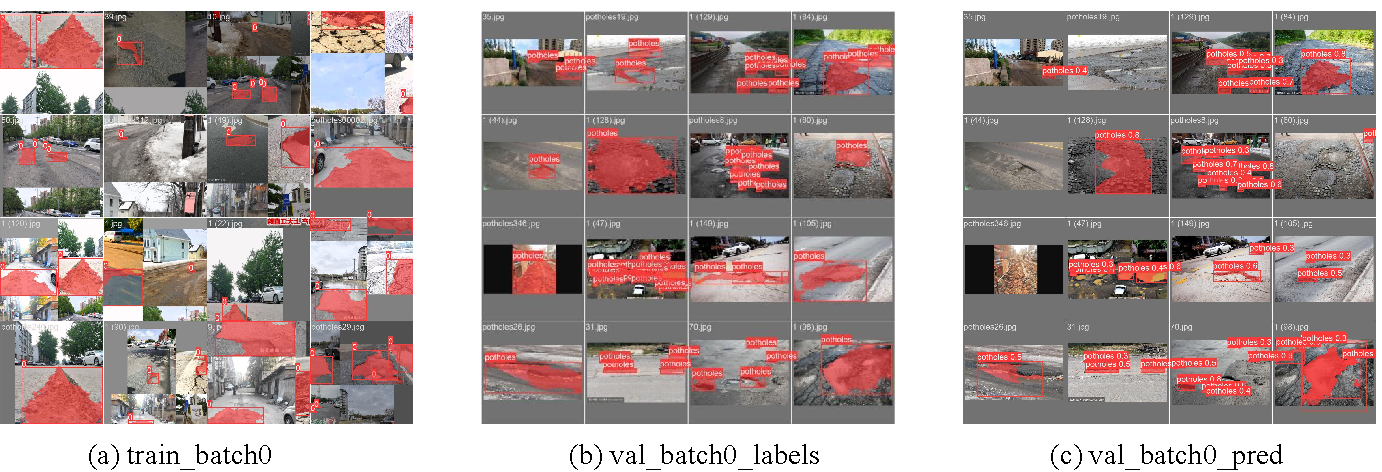
\includegraphics[scale=0.5]{Figures/segment/Segment训练.pdf}
			\caption{YOLOv8s-Segment训练数据集增强}
			\label{fig:YOLOv8s-Segment训练数据集增强}
		\end{figure}

		训练过程的每一次迭代的结果保存于“支撑材料/process/训练”文件夹中。训练结束后,会生成“best.pt”与“last.pt”模型文件,我们选择“best.pt”作为后续预测的图像分割模型。而对于模型的效果分析,详见\textcolor{blue}{\nameref{模型效果分析}}。
		\item \textbf{YOLOv8n-Detect}
		
		对于该模型的训练与上述模型类似。在训练时,其也会生成数据集的相关特征,如\textcolor{blue}{\cref{fig:YOLOv8n-Detect训练数据集特征}}所示。
		\begin{figure}[H]
			\centering
			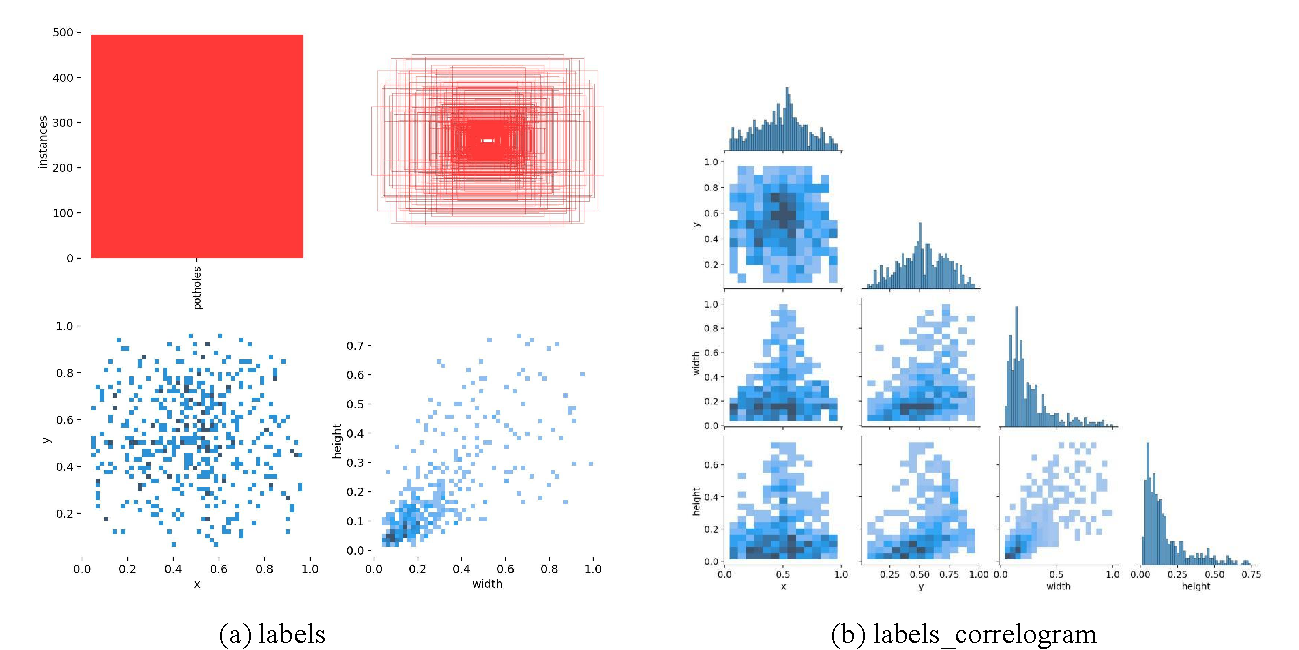
\includegraphics[scale=0.5]{Figures/detect/DetectLabels.pdf}
			\caption{YOLOv8n-Detect训练数据集特征}
			\label{fig:YOLOv8n-Detect训练数据集特征}
		\end{figure}

		在训练过程中,模型也将对数据进行增强,部分效果如\textcolor{blue}{\cref{fig:YOLOv8n-Detect训练数据集增强}}所示,由于篇幅原因,其余的详见附录。
		\begin{figure}[H]
			\centering
			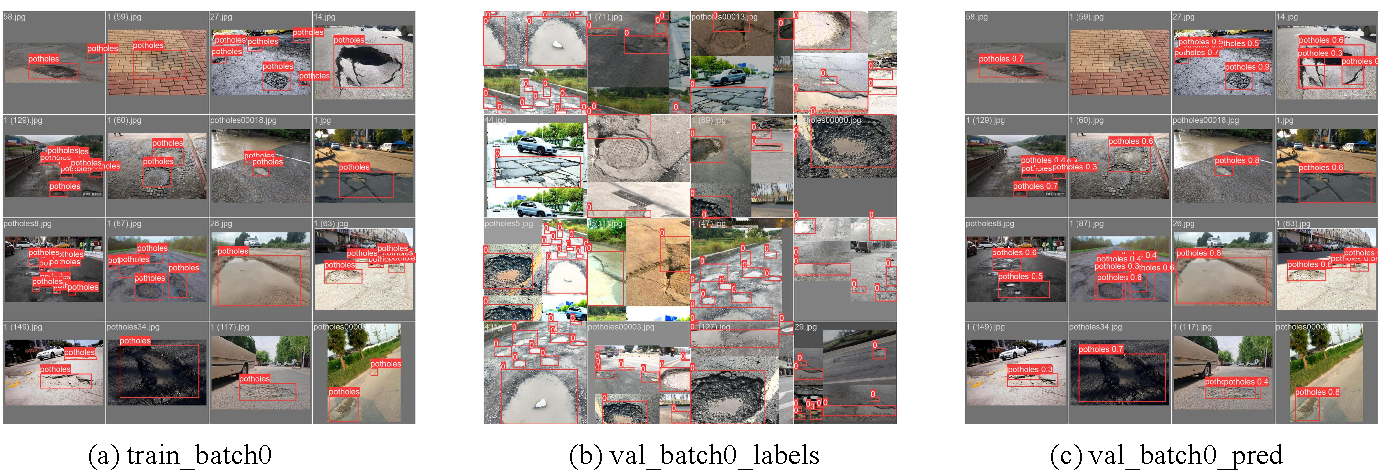
\includegraphics[scale=0.5]{Figures/detect/Detect训练.pdf}
			\caption{YOLOv8n-Detect训练数据集增强}
			\label{fig:YOLOv8n-Detect训练数据集增强}
		\end{figure}

		训练过程的每一次迭代的结果保存于“支撑材料/process/训练”文件夹中。训练结束后,会生成“best.pt”与“last.pt”模型文件,我们选择“best.pt”作为后续预测的图像检测模型。而对于模型的效果分析,详见\textcolor{blue}{\nameref{模型效果分析}}。
	\end{itemize}
	\subsection{测试集图像坑洼特性预测}\label{预测}
	在对测试集图像坑洼特性预测前,首先要判断各图像文件是否能够读取,在\textcolor{blue}{\nameref{预读取}}中,经测试有一文件读取失败,读入的数组为空,将会导致后续批量预测的中断。这里我们考虑到,在系统中能够正常打开,而利用opencv或pillow库均打开失败。因此,我们考虑尝试重新另存为该张图片为JPG格式文件,再重新读取。经过测试,通过上述操作后,文件能够正常读取,且信息正确。至此4942张图片均能正常读取,方便后续批量、统一预测。
	\subsubsection{道路坑洼的边缘提取}
	利用上述训练好的模型,可以对未知数据集进行批量预测,提取其坑洼的边缘,现随机挑选一张图片,文件名为“em5acvux.jpg”,结果见\textcolor{blue}{\cref{fig:效果展示}}。可以发现,无论是图像分割还是图像检测,其均能较好地提取出坑洼的边缘信息,但图像分割的效果更好,其能够更好地提取出坑洼的边缘,且能够将坑洼的形态进行较好的还原。
	\begin{figure}[H]
		\centering
		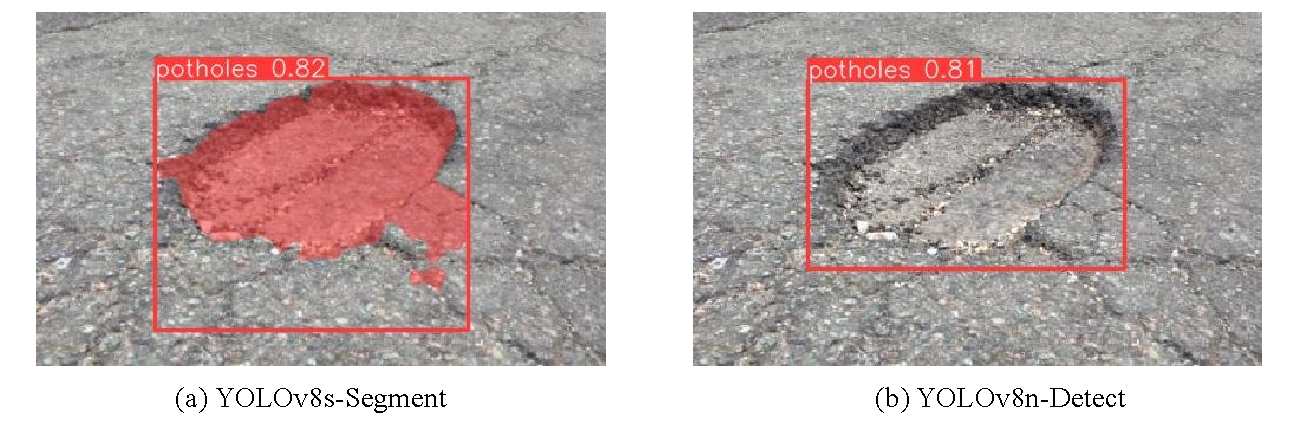
\includegraphics[scale=0.5]{效果展示.pdf}
		\caption{效果展示}
		\label{fig:效果展示}
	\end{figure}
	对于上述起初读取失败的“guy7iodk.jpg”文件,这里我们也将结果展示,如\textcolor{blue}{\cref{fig:guy7iodk结果展示}}所示。观察该图,我们可以发现,YOLOv8s-Segment模型能够较好地提取出坑洼的边缘,但YOLOv8n-Detect模型提取的坑洼边缘信息不够完整,且存在一定的误差。
	\begin{figure}[H]
		\centering
		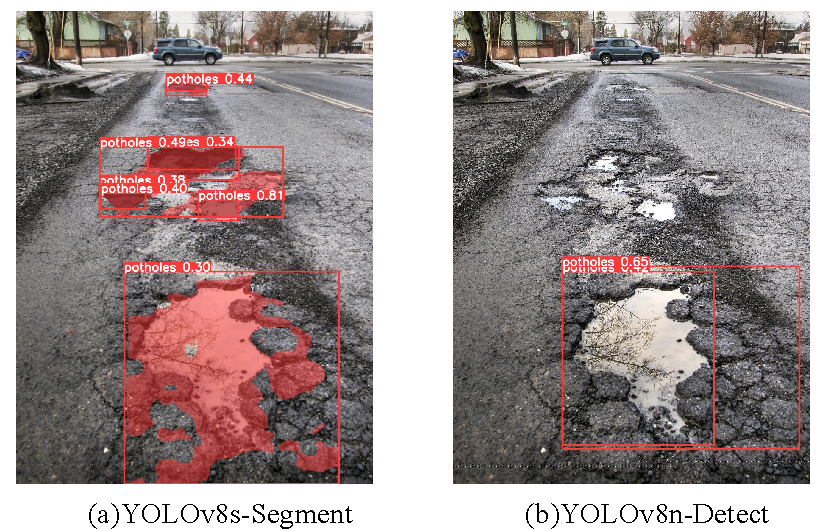
\includegraphics[scale=0.5]{guy7iodk结果展示.pdf}
		\caption{guy7iodk.jpg结果展示}
		\label{fig:guy7iodk结果展示}
	\end{figure}
	\subsubsection{道路坑洼的面积占比估算}
	由于坑洼的形态多样,在对使用图像检测的矩形计算其面积占比时,需要考虑到以下五种基本情况,其有着不同的处理方法,以下进行具体叙述,记坑洼面积占原图像面积比值为$\eta\,\%$\textcolor{blue}{\footnote{本文计算的$\eta$均向上取整。}}。在估算面积占比之前,需要利用之前训练好的模型对未知数据集图像文件进行预测,得到坑洼的边框相对坐标信息。但由于在估算时,需要使用到绝对坐标信息,因此,我们需要对其进行转换。这里我们使用Python进行处理,具体处理代码见\textbf{附录-C.10,Coordinate Transformation [坐标转换]}。
	\begin{itemize}
		\item \textbf{图中无坑洼};在模型预测时,其支持输出预测的图像中坑洼的个数,利用Python的pandas库将其进行处理,即可得到各图预测的坑洼个数。当坑洼个数为0时,面积占比为0。
		\item \textbf{图中仅有一处坑洼};当图中仅有一处坑洼时,可以直接计算该坑洼的面积,从而求得其占比。如\textcolor{blue}{\cref{fig:单一坑洼面积占比估算示意图}}所示。
		\begin{figure}[H]
			\centering
			\begin{minipage}{0.45\linewidth}
			  \centering
			  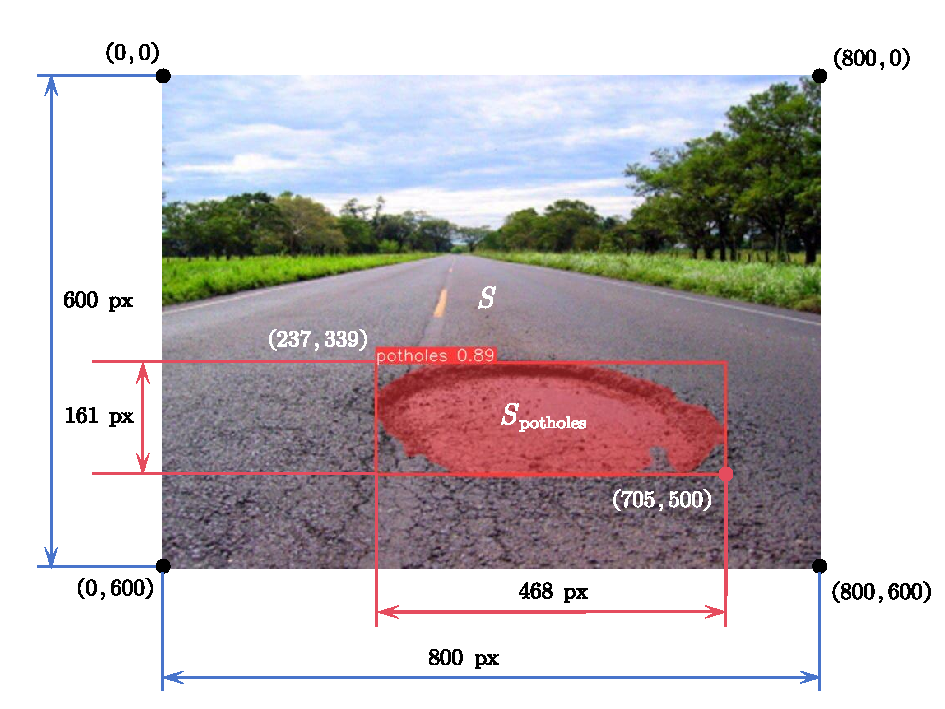
\includegraphics[width=1.0\linewidth]{单一坑洼面积占比估算示意图.pdf}
			  \caption{单一坑洼面积占比估算示意图}
			  \label{fig:单一坑洼面积占比估算示意图}
			\end{minipage}
			%qquad
			\begin{minipage}{0.45\linewidth}
			  \centering
			  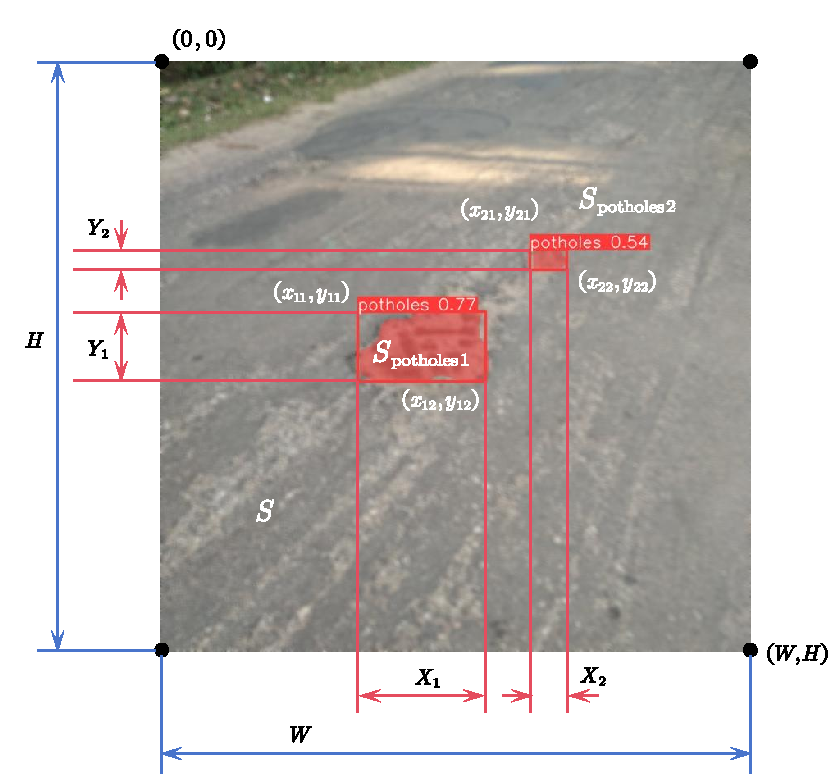
\includegraphics[width=0.77\linewidth]{多个不重叠坑洼面积占比估算示意图.pdf}
			  \caption{多个不重叠坑洼面积占比估算示意图}
			  \label{fig:多个不重叠坑洼面积占比估算示意图}
			\end{minipage}
		\end{figure}
		定义图像长、宽的像素值分别为$W$、$H$。则图像面积为:
		\begin{equation}
			S=W\cdot H
		\end{equation}
		
		在图像坐标系中,左上角为原点,记坑洼边框的左上角坐标为$\left(x_1,y_1\right)$,右下角坐标为$\left(x_2,y_2\right)$,坑洼的长、宽的像素值分别为$X$,$Y$,则坑洼的面积为:
		\begin{equation}
			S_{\text{potholes}}=X\cdot Y=\left(x_2-x_1\right)\cdot\left(y_2-y_1\right)
		\end{equation}
		
		因此坑洼面积占比为:
		\begin{equation}
			\eta=\frac{S_{\text{potholes}}}{S}\times 100
		\end{equation}
		
		例如\textcolor{blue}{\cref{fig:单一坑洼面积占比估算示意图}}的长、宽的像素值分别为$W=800$,$H=600$,坑洼的长、宽的像素值分别为$X=468$,$Y=161$,则坑洼面积占比为:
		\begin{equation}
			\eta=\frac{468\times 161}{800\times 600}\times 100=16
		\end{equation}
		\item \textbf{图中有多个坑洼,但两两互不重叠}:该种情况,如\textcolor{blue}{\cref{fig:多个不重叠坑洼面积占比估算示意图}}所示。其处理方法与图中仅有一处坑洼类似,首先计算各坑洼的面积,然后求和,即可得到坑洼面积占比,即:
		\begin{equation}
			\eta=\frac{\sum\limits_{i=1}^nS_{\text{potholes},i}}{S}\times 100=\frac{\sum\limits_{i=1}^n\left[\left(x_{i2}-x_{i1}\right)\cdot\left(y_{i2}-y_{i1}\right)\right]}{W\cdot H}\times 100
		\end{equation}
		\item \textbf{图中有两坑洼为包含关系}:当坑洼为包含关系时,不可简单对其进行求和,而应以最大的坑洼面积作为总的坑洼面积,如\textcolor{blue}{\cref{fig:完全重叠坑洼面积占比估算示意图}}即:
		\begin{equation}
			\eta=\frac{\max\limits_{i=1}^nS_{\text{potholes},i}}{S}\times 100=\frac{\max\limits_{i=1}^n\left[\left(x_{i2}-x_{i1}\right)\cdot\left(y_{i2}-y_{i1}\right)\right]}{W\cdot H}\times 100
		\end{equation}
		\begin{figure}[H]
			\centering
			\begin{minipage}{0.45\linewidth}
			  \centering
			  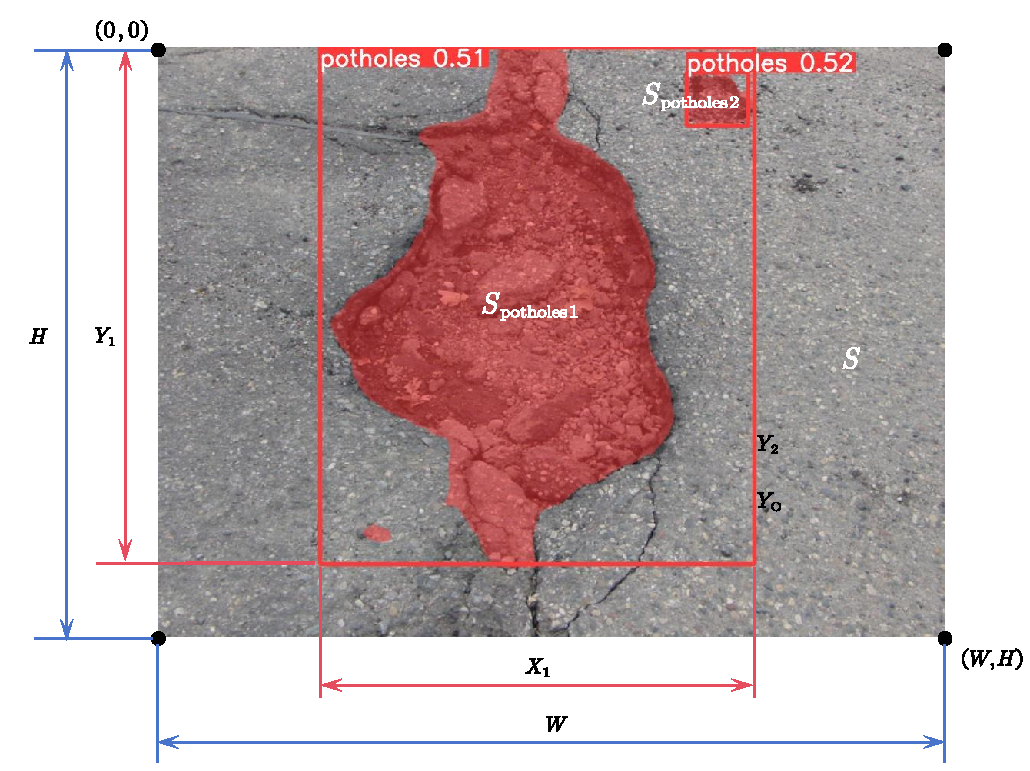
\includegraphics[width=0.99\linewidth]{完全重叠坑洼面积占比估算示意图.pdf}
			  \caption{完全重叠坑洼面积占比估算示意图}
			  \label{fig:完全重叠坑洼面积占比估算示意图}
			\end{minipage}
			%qquad
			\begin{minipage}{0.45\linewidth}
			  \centering
			  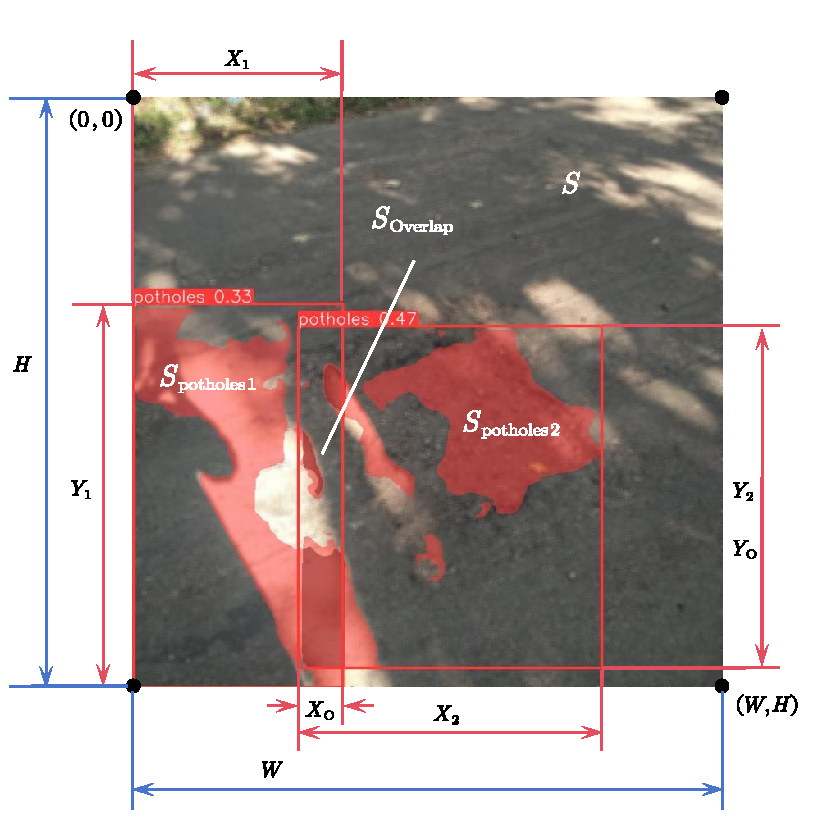
\includegraphics[width=0.74\linewidth]{部分重叠坑洼面积占比估算示意图.pdf}
			  \caption{部分重叠坑洼面积占比估算示意图}
			  \label{fig:部分重叠坑洼面积占比估算示意图}
			\end{minipage}
		\end{figure}
		\item \textbf{图中有两坑洼部分重叠}:对于该情况,如\textcolor{blue}{\cref{fig:部分重叠坑洼面积占比估算示意图}}所示。基本方法是,先求得各坑洼的面积,然后求和,最后减去重叠部分的面积,即:
		\begin{equation}
			\eta=\frac{\sum\limits_{i=1}^nS_{\text{potholes},i}-\sum S_{\text{overlap}}}{S}\times 100=\frac{\sum\limits_{i=1}^n\left[\left(x_{i2}-x_{i1}\right)\cdot\left(y_{i2}-y_{i1}\right)\right]-\sum S_{\text{overlap}}}{W\cdot H}\times 100
		\end{equation}
	
		对于$S_{\text{overlap}}$的计算,需要分如\textcolor{blue}{\cref{fig:部分重叠四种情况}}所示的四种情况。
		\begin{figure}[H]
			\centering
			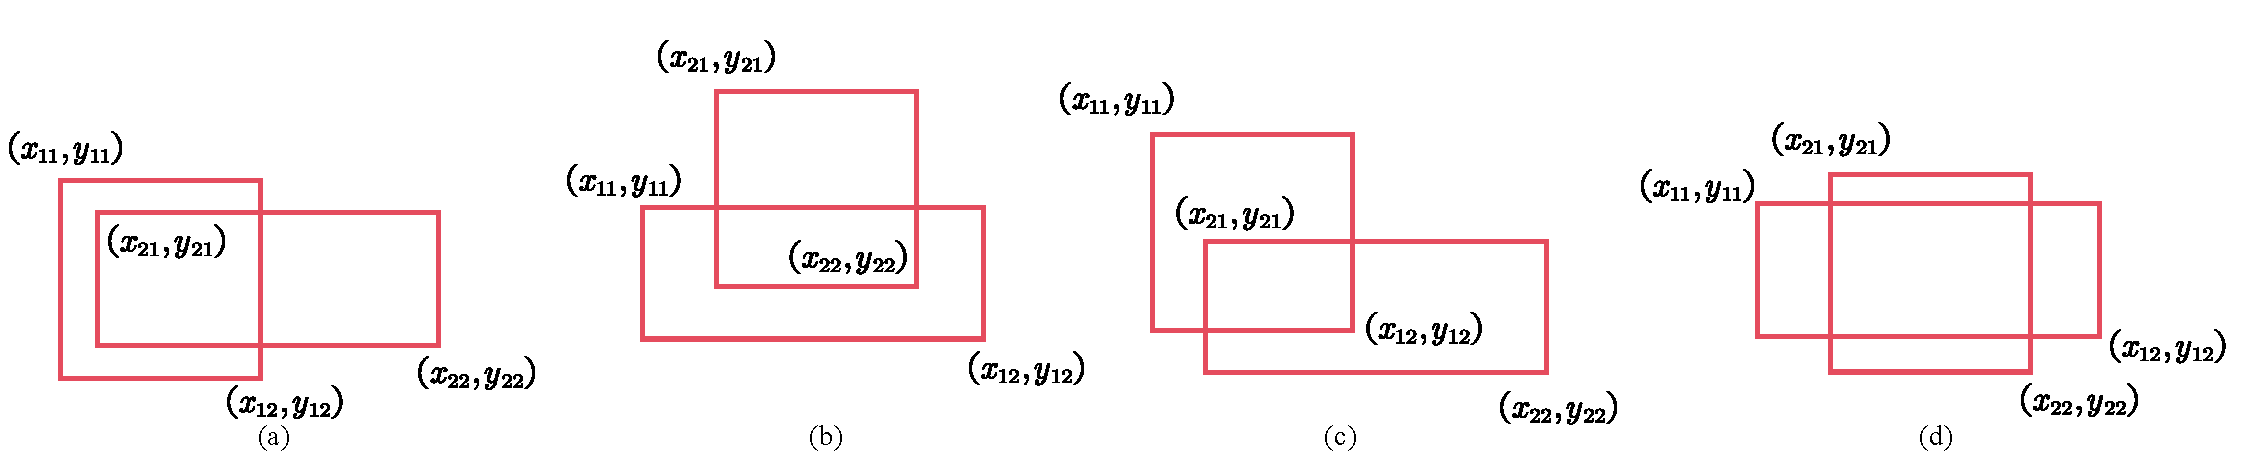
\includegraphics[scale=0.4]{部分重叠四种情况.pdf}
			\caption{部分重叠四种情况}
			\label{fig:部分重叠四种情况}
		\end{figure}
		\begin{itemize}
			\item \textbf{a}
			\begin{equation}
				S_{\text{overlap}}=\left(x_{12}-x_{21}\right)\cdot\left(y_{22}-y_{21}\right)
			\end{equation}
			\item \textbf{b}
			\begin{equation}
				S_{\text{overlap}}=\left(x_{22}-x_{21}\right)\cdot\left(y_{22}-y_{11}\right)
			\end{equation}
			\item \textbf{c}
			\begin{equation}
				S_{\text{overlap}}=\left(x_{12}-x_{21}\right)\cdot\left(y_{12}-y_{21}\right)
			\end{equation}
			\item \textbf{d}
			\begin{equation}
				S_{\text{overlap}}=\left(x_{22}-x_{21}\right)\cdot\left(y_{12}-y_{11}\right)
			\end{equation}
		\end{itemize}
	\end{itemize}

	此外,由于坑洼图像的多样、复杂,部分图片可能存在上述基本情况的综合,因此,对于每一情况,均需要特定计算,再求和,从而求得其占比。
	
	经过上述分析,整合如\textcolor{blue}{\cref{tab:道路坑洼面积占比估算计算数据集}}所示的数据集。表中仅罗列出了部分数据,且部分文件存在多行,这是由于其存在多个坑洼,因此,需要逐个文件进行处理。
\begin{table}[H]
	\centering
	\caption{道路坑洼面积占比估算计算数据集}
	\scalebox{0.7}{
	  \begin{tabular}{rrrrrrrrrr}
	  \toprule
	  \textbf{索引} & \textbf{fnames} & \textbf{置信度} & $x_1$ & $y_1$ & $x_2$ & $y_2$ & \textbf{Npotholes} & \textbf{height} & \textbf{width} \\
	  \midrule
	  0     & 00c9sdfq.jpg & 0.783255  & 54.144627  & 119.418549  & 127.293488  & 149.223495  & 2     & 259   & 194 \\
	  1     & 00c9sdfq.jpg & 0.727551  & 86.166367  & 92.886162  & 143.883499  & 117.423920  & 2     & 259   & 194 \\
	  2     & 00yf8rxj.jpg & 0.685144  & 0.000000  & 268.575745  & 714.198425  & 439.384949  & 1     & 450   & 800 \\
	  3     & 01lx7dej.jpg & 0.345122  & 723.983704  & 628.620300  & 1671.653564  & 1621.744507  & 1     & 3264  & 2448 \\
	  4     & 01paoyy0.jpg & 0.447922  & 62.188206  & 54.767998  & 338.213837  & 239.532608  & 1     & 300   & 447 \\
	  …     & …     & …     & …     & …     & …     & …     & …     & …     & … \\
	  6506  & zynixpux.jpg & 0.266729  & 55.626934  & 116.560684  & 126.989532  & 136.572723  & 3     & 300   & 481 \\
	  6507  & zyylqfs0.jpg & 0.829763  & 645.354004  & 481.915741  & 1075.006836  & 717.232178  & 1     & 816   & 1200 \\
	  6508  & zzhe6767.jpg & NaN   & NaN   & NaN   & NaN   & NaN   & 0     & 555   & 986 \\
	  6509  & zzipq9zn.jpg & NaN   & NaN   & NaN   & NaN   & NaN   & 0     & 300   & 463 \\
	  6510  & zzvomOax.jpg & 0.711966  & 0.000822  & 369.854126  & 1447.335327  & 984.154907  & 1     & 1080  & 1623 \\
	  \bottomrule
	  \end{tabular}}
	\label{tab:道路坑洼面积占比估算计算数据集}
  \end{table}
  现依据该表及上述分析对各图中坑洼占比进行计算,处理代码详见\textbf{附录-C.11,Proportional Calculation [面积占比估算]}。

	\begin{itemize}
		\item \textbf{读取已建立、训练完成的模型}:将上述CNN-SVM模型利用keras及pickle库读取;
		\item \textbf{读取未知数据集}:将未知数据集的图像数据及其文件名(包括后缀名)一并读入,方便后续结果的输出,共计4942张图像;
		\item \textbf{对未知数据集进行预处理}:为了准确预测,需要将该数据集格式转换为前期训练模型输入的格式,避免预测错误。
		\item \textbf{对未知数据集进行预测}:首先传入CNN卷积神经网络,对数据集的特征进行提取;之后将提取的特征数据集传入SVM支持向量机中,进行预测;
		\item \textbf{结果查看}:经过上述步骤,将文件名与预测结果一一对应转为表格数据,方便查看;通过预测,模型在4942张图像中,识别出坑洼道路为3765张,识别为正常道路为1177张。
		\item \textbf{保存结果}:确认无误后,将上述表格输出为“test\_result.csv”文件。
	\end{itemize}

	\subsection{模型的评估}\label{模型效果分析}
	\subsubsection{模型评估指标}
	为更好地评估模型,我们针对上述模型进行多维度评估,这里我们用到的有:
	\begin{itemize}
		\item \textbf{损失值(Loss)}:损失函数由预测的中心坐标损失、预测边界框的宽高损失、预测的类别损失、预测的置信度损失四个部分组成\textcolor{blue}{\cite{LOSS}}。
		\begin{itemize}
			\item {\heiti 中心坐标损失}:
		\begin{equation}
			L_1=\lambda_{\text{coord}}\sum\limits_{i=0}^{S^2}\sum\limits_{j=0}^{B}\mathcal{l}_{ij}^{\text{obj}}\left[\left(x_i-\hat{x}_i\right)^2+\left(y_i-\hat{y}_i\right)^2\right]
		\end{equation}
		该式计算了相对于预测的边界框位置$\left(x,y\right)$的损失值。定义当$\mathcal{l}_{ij}^{\text{obj}}$的值为$1$时,如果网格单元$i$中存在目标,则第$j$个边界框预测值对该预测有效。
			\item {\heiti 预测边界框的宽高损失}:
			\begin{equation}
				L_2=\lambda_{\text{coord}}\sum\limits_{i=0}^{S^2}\sum\limits_{j=0}^{B}\mathcal{l}_{ij}^{\text{obj}}\left[\left(\sqrt{w_i}-\sqrt{\hat{w}_i}\right)^2+\left(\sqrt{h_i}-\sqrt{\hat{h}_i}\right)^2\right]
			\end{equation}
			\item {\heiti 预测类别损失}:
			\begin{equation}
				L_3=\sum\limits_{i=0}^{S^2}\mathcal{l}_{i}^{\text{obj}}\sum\limits_{c\in\text{classes}}\left[p_i\left(c\right)-\hat{p}_i\left(c\right)\right]^2
			\end{equation}
			\item {\heiti 预测置信度损失}:
			\begin{equation}
				L_4=\sum\limits_{i=0}^{S^2}\sum\limits_{j=0}^{B}\mathcal{l}_{ij}^{\text{obj}}\left(C_i-\hat{C}_i\right)^2+\lambda_{\text{noobj}}\sum\limits_{i=0}^{S^2}\sum\limits_{j=0}^{B}\mathcal{l}_{ij}^{\text{noobj}}\left(C_i-\hat{C}_i\right)^2
			\end{equation}
			其中$C$为置信度得分,$\hat{C}$是预测边界框与基本事实的交叉部分。当一个单元格有对象时,$\mathcal{l}_{i}^{\text{obj}}$为1,否则为0。
			\end{itemize}
			因此损失值为:
			\begin{equation}
				L=L_1+L_2+L_3+L_4
			\end{equation}
		\item \textbf{精确率(Precision)、召回率(Recall),F1分数值(F1-Score)}:
		\begin{itemize}
			\item {\heiti 精确率}
			\begin{equation}
				\mathrm{Precision} = \frac{TP}{TP+FP} \label{Precision}
			\end{equation}
			\item {\heiti 召回率}
			\begin{equation}
				\mathrm{Recall} = \frac{TP}{TP+FN} \label{Recall}
			\end{equation}
			\item {\heiti F1分数值} 
			\begin{equation}
				\mathrm{F}1 = \frac{2\times \mathrm{Precision}\times \mathrm{Recall}}{\mathrm{Precision}+\mathrm{Recall}}=\frac{TP}{TP+\frac{1}{2}\left(FP+FN\right)} \label{F1-Score}
			\end{equation}
		\end{itemize}
		对于$TP$、$FN$、$FP$、$TN$,其中T为True,F为False,这两个字母表示预测值与实际值是否相同;P为Positive,N为Negative,这两个字母表示预测出的是属于正类还是负类。因此$TP$为预测为正类且实际为正类的样本数,$FN$为预测为负类且实际为正类的样本数,$FP$为预测为正类且实际为负类的样本数,$TN$为预测为负类且实际为负类的样本数。

		此外,对于模型的精确率、召回率,我们可以根据定义可以发现若这两项值较大,则模型效果较好。同时根据定义,我们可以发现模型的精确率、召回率在理想情况下是相差较小的,我们可以根据图示结果验证,符合预期效果。对于模型的F1分数值,其为精确率与召回率的调和平均数\textcolor{blue}{\cite{模型评测}},因此当精确率与召回率均有较好表现时,F1分数值会有较优秀表现。我们也可对\textcolor{blue}{\eqref{F1-Score}}进行一定变换,可以得到:
		\begin{equation}
			\mathrm{F}1=\frac{2}{\dfrac{1}{\mathrm{Precision}}+\dfrac{1}{\mathrm{Recall}}} \label{ReacllNew}
		\end{equation}
		根据该式,我们可以得出上述结论。

		\item \textbf{混淆矩阵(Confusion Matrix)}:矩阵每一行表示样本标签的实际类别,在本题中表示道路类型:为正常还是坑洼的实际标签;每一列表示样本标签的预测类别,在本题中表示道路类型:为正常还是坑洼的预测标签。因此该图示的主对角线数据之和即为模型预测准确的样本数。这里此外还需要引入四项值,而混淆矩阵可以直观地观察到预测准确与错误的情况,以及模型对于每一类别的区分程度。
		\item \textbf{精确率-召回率曲线(Precision-Recall Curve,PR-Curve)}:该图像可表现出分类的预测精度与召回率之间的关系\textcolor{blue}{\cite{Yellowbrick}}。图像的填充区域越大,分类效果越优。
		\item \textbf{mAP}:其中AP是某一类别的精确率-召回率
		曲线(PR-Curve)下的面积,而mAP则是计算所有类别的PR曲
		线下面积的平均值,即:
		\begin{equation}
			\mathrm{AP}=\sum\limits_{i=1}^n\left(\mathrm{R}_i-\mathrm{R}_{i-1}\right)\mathrm{P}_i
		\end{equation}
		\begin{equation}\label{mAP}
			\mathrm{mAP}=\frac{1}{Q}\sum\limits_{q=1}^Q\mathrm{AP}\left(q\right)
		\end{equation}
		在本题中,由于我们只研究道路坑洼,因此mAP与AP是相等的,即\textcolor{blue}{\eqref{mAP}}中$Q=1$。
		\item \textbf{mAP50}:$50$表示目标的交集与并集之比IoU(Intersection over Union)阈值为$50$,即当预测框与真实框的IoU大于$50\%$时,该预测框为正确预测框。若记真实区域为$A$,预测区域为$B$,则IoU为:
		\begin{equation}
			\mathrm{IoU}=\frac{A\cap B}{A\cup B}
		\end{equation}
		\item \textbf{mAP50-95}:$50-95$表示mAP阈值为50到mAP阈值为95,间隔5,取得10个mAP值,再对这十个值取平均\textcolor{blue}{\cite{指标}}。
		\item \textbf{epoch过程中各项指标变化图}:该图可直观地观察到模型在训练过程中各项指标的变化情况,从而判断模型是否收敛,以及模型的收敛速度。
	\end{itemize}
	\subsubsection{YOLOv8s-Segment}
	对于图像分割模型,绘制其Box及Mask,即该模型会对坑洼标注矩形框的同时也会标注其边缘信息,如\textcolor{blue}{\cref{fig:YOLOv8s-Segment-Box}}及\textcolor{blue}{\cref{fig:YOLOv8s-Segment-Mask}}所示。
	\begin{figure}[H]
		\centering
		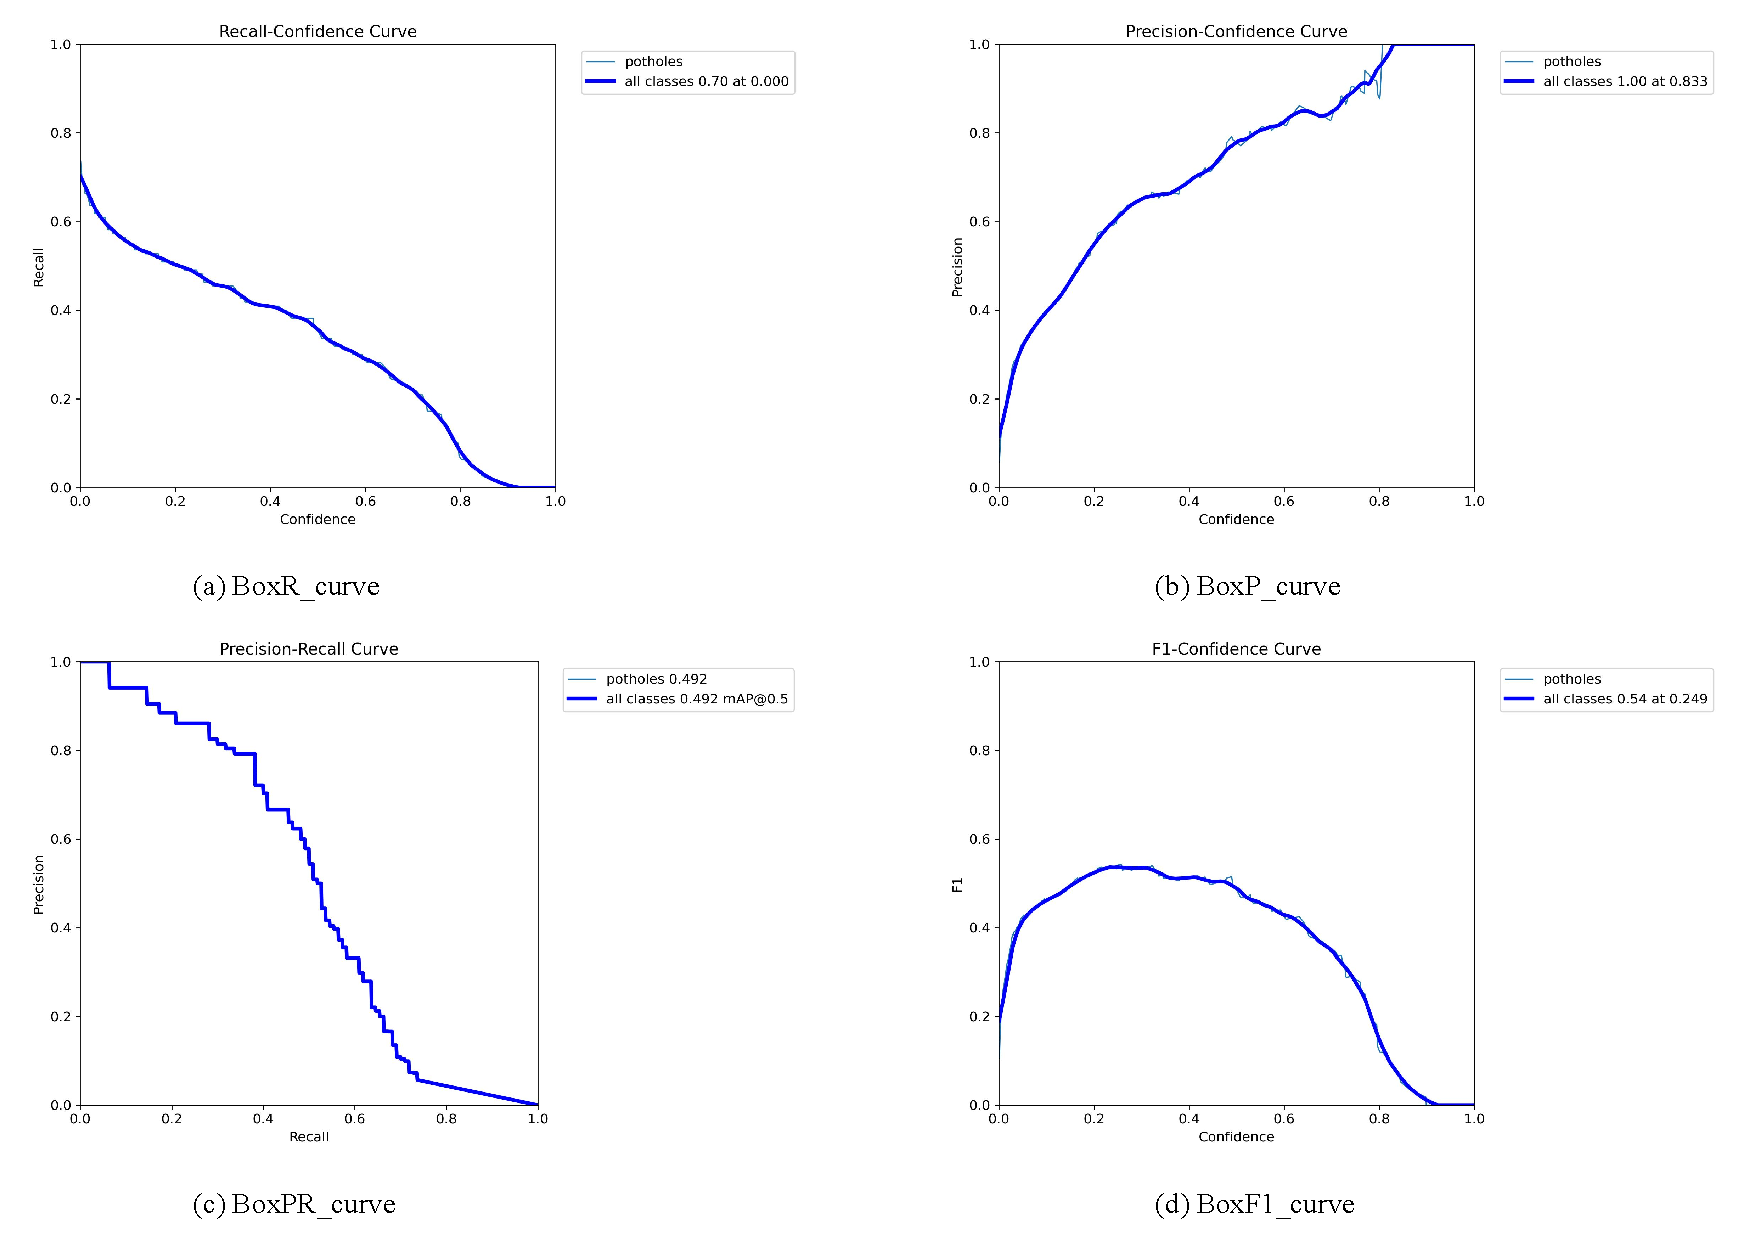
\includegraphics[scale=0.5]{Figures/segment/SegmentBox.pdf}
		\caption{YOLOv8s-Segment Box}
		\label{fig:YOLOv8s-Segment-Box}
	\end{figure}
	\begin{figure}[H]
		\centering
		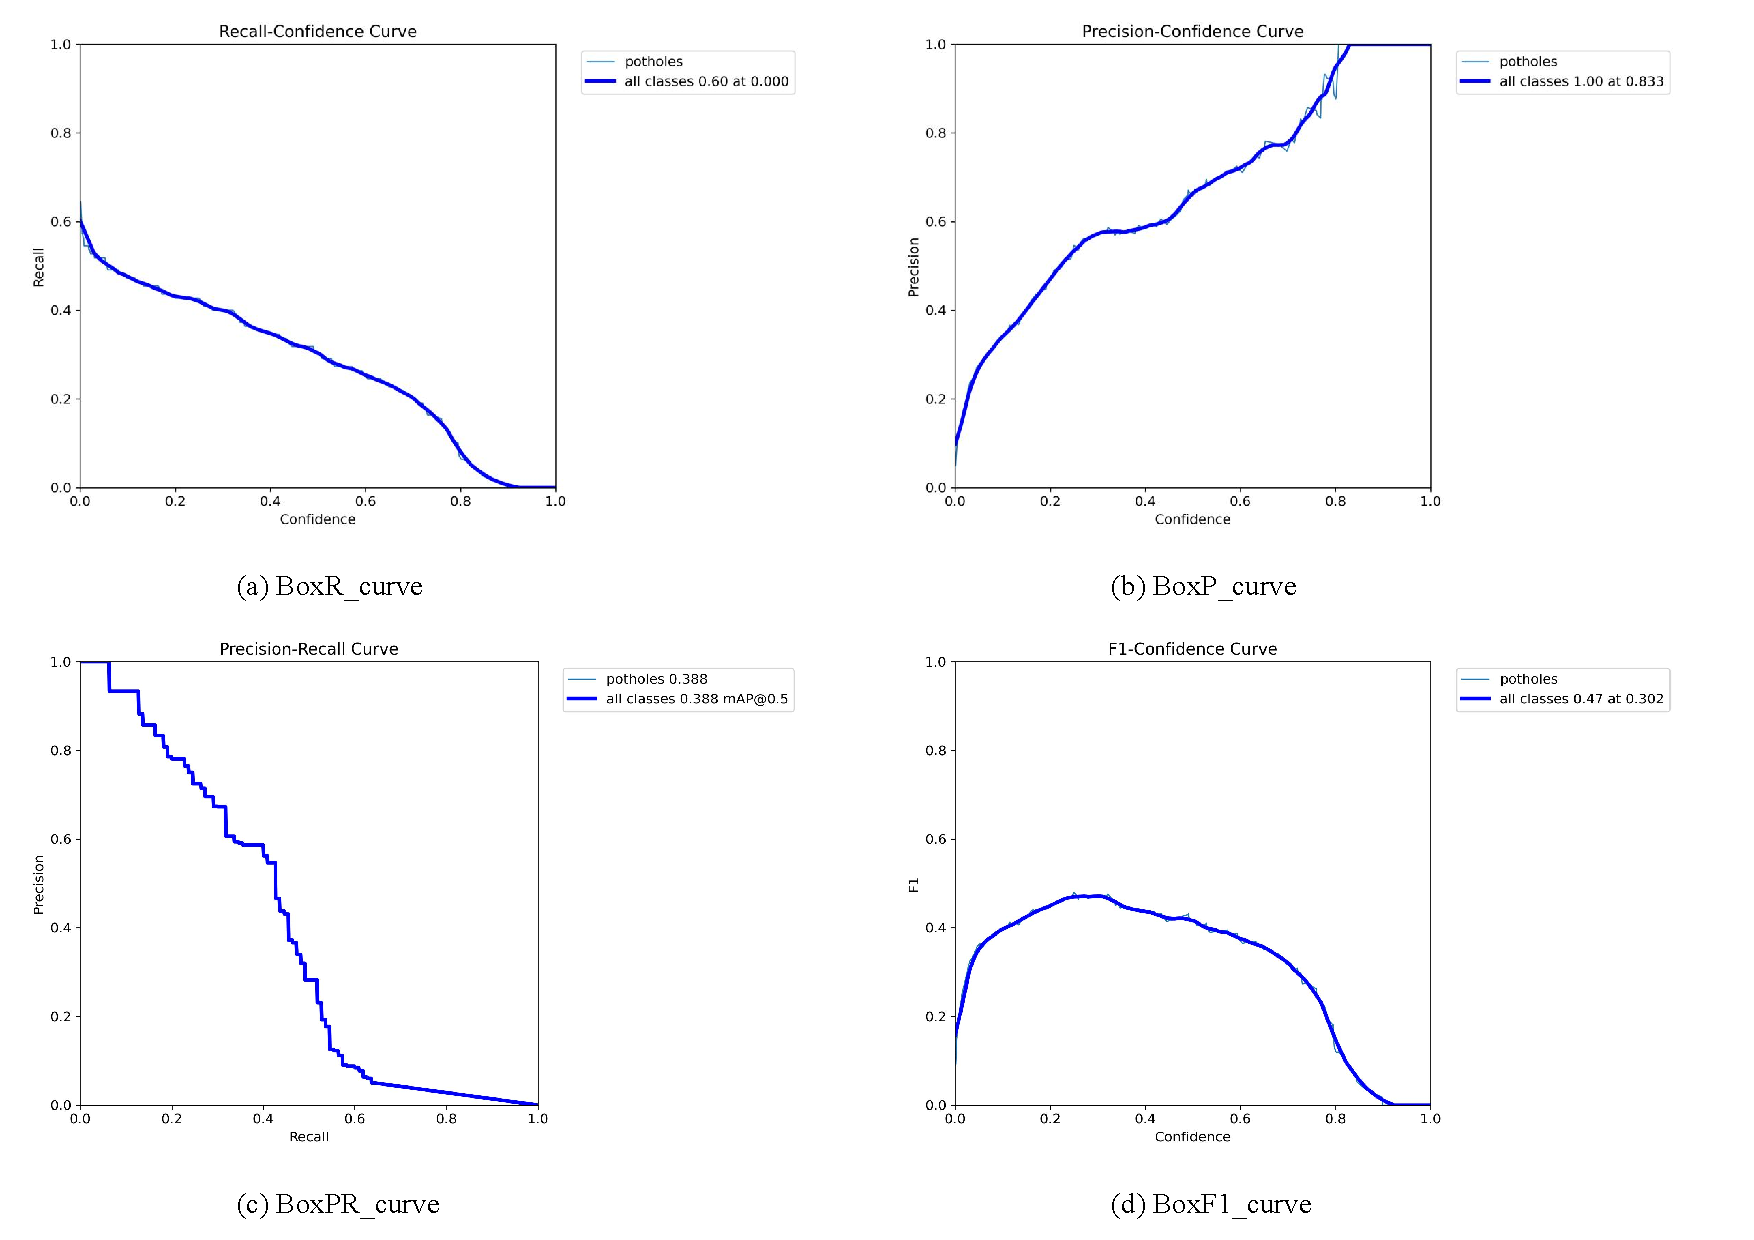
\includegraphics[scale=0.5]{Figures/segment/SegmentMask.pdf}
		\caption{YOLOv8s-Segment Mask}
		\label{fig:YOLOv8s-Segment-Mask}
	\end{figure}
	观察上述图示,可以发现各项指标在Box中较为优秀,而在Mask中相对较低,这是由于在标注矩形框时,仅需要坑洼的最边界信息,而无需具体到其轮廓、形态等特征。而边缘分割时,需要获取其边缘信息,需要具体到其轮廓、形态等特征,因此该任务相对于Box标注更为困难,因此其指标相对较低。

	同时,绘制模型的混淆矩阵热力图,如\textcolor{blue}{\cref{fig:YOLOv8s-Segment-ConfusionMatrix}}所示,采用两种计算,其一为数量统计,其二为数据标准化统计。可以发现对于坑洼的识别,其坑洼预测正确率为$0.51\,\%$,对于background并未进行训练,因此表现出的效果较差。考虑到各坑洼的轮廓、形态、所在区域的多样及复杂,其预测效果仍可以接受。但出于未来模型的改进,我们仍需要对其进行改进,以提高其预测效果,在模型的评价中,我们也将进行一定叙述。
	\begin{figure}[H]
		\centering
		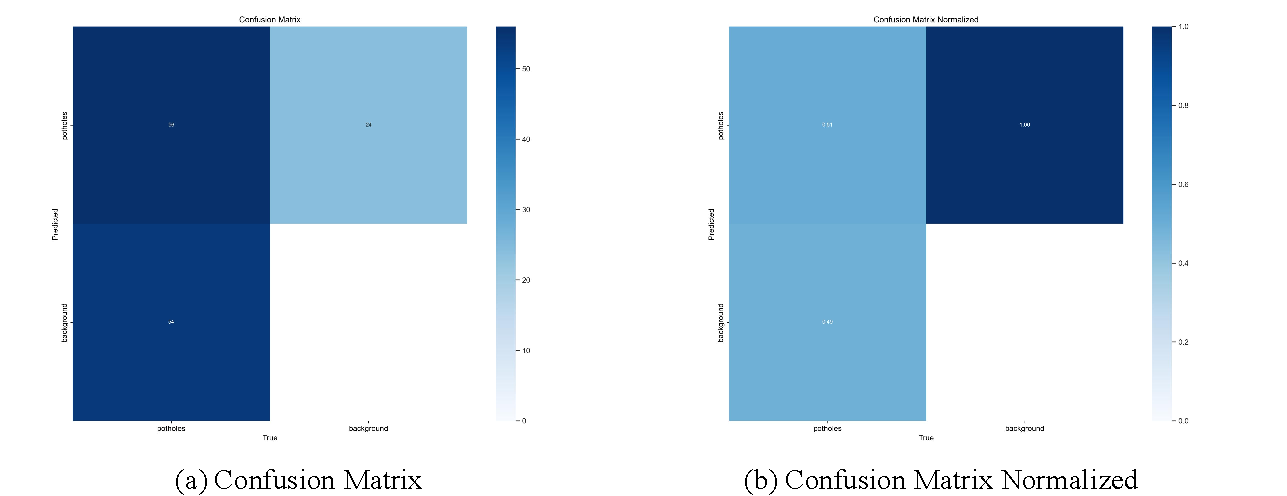
\includegraphics[scale=0.66]{Figures/segment/SegmentConfusionMatrix.pdf}
		\caption{YOLOv8s-Segment Confusion Matrix}
		\label{fig:YOLOv8s-Segment-ConfusionMatrix}
	\end{figure}
	
	此外,绘制训练过程中每一次Epoch的各项指标,如\textcolor{blue}{\cref{fig:YOLOv8s-Segment-Results}}所示。观察该图,我们可以发现
	\begin{figure}[H]
		\centering
		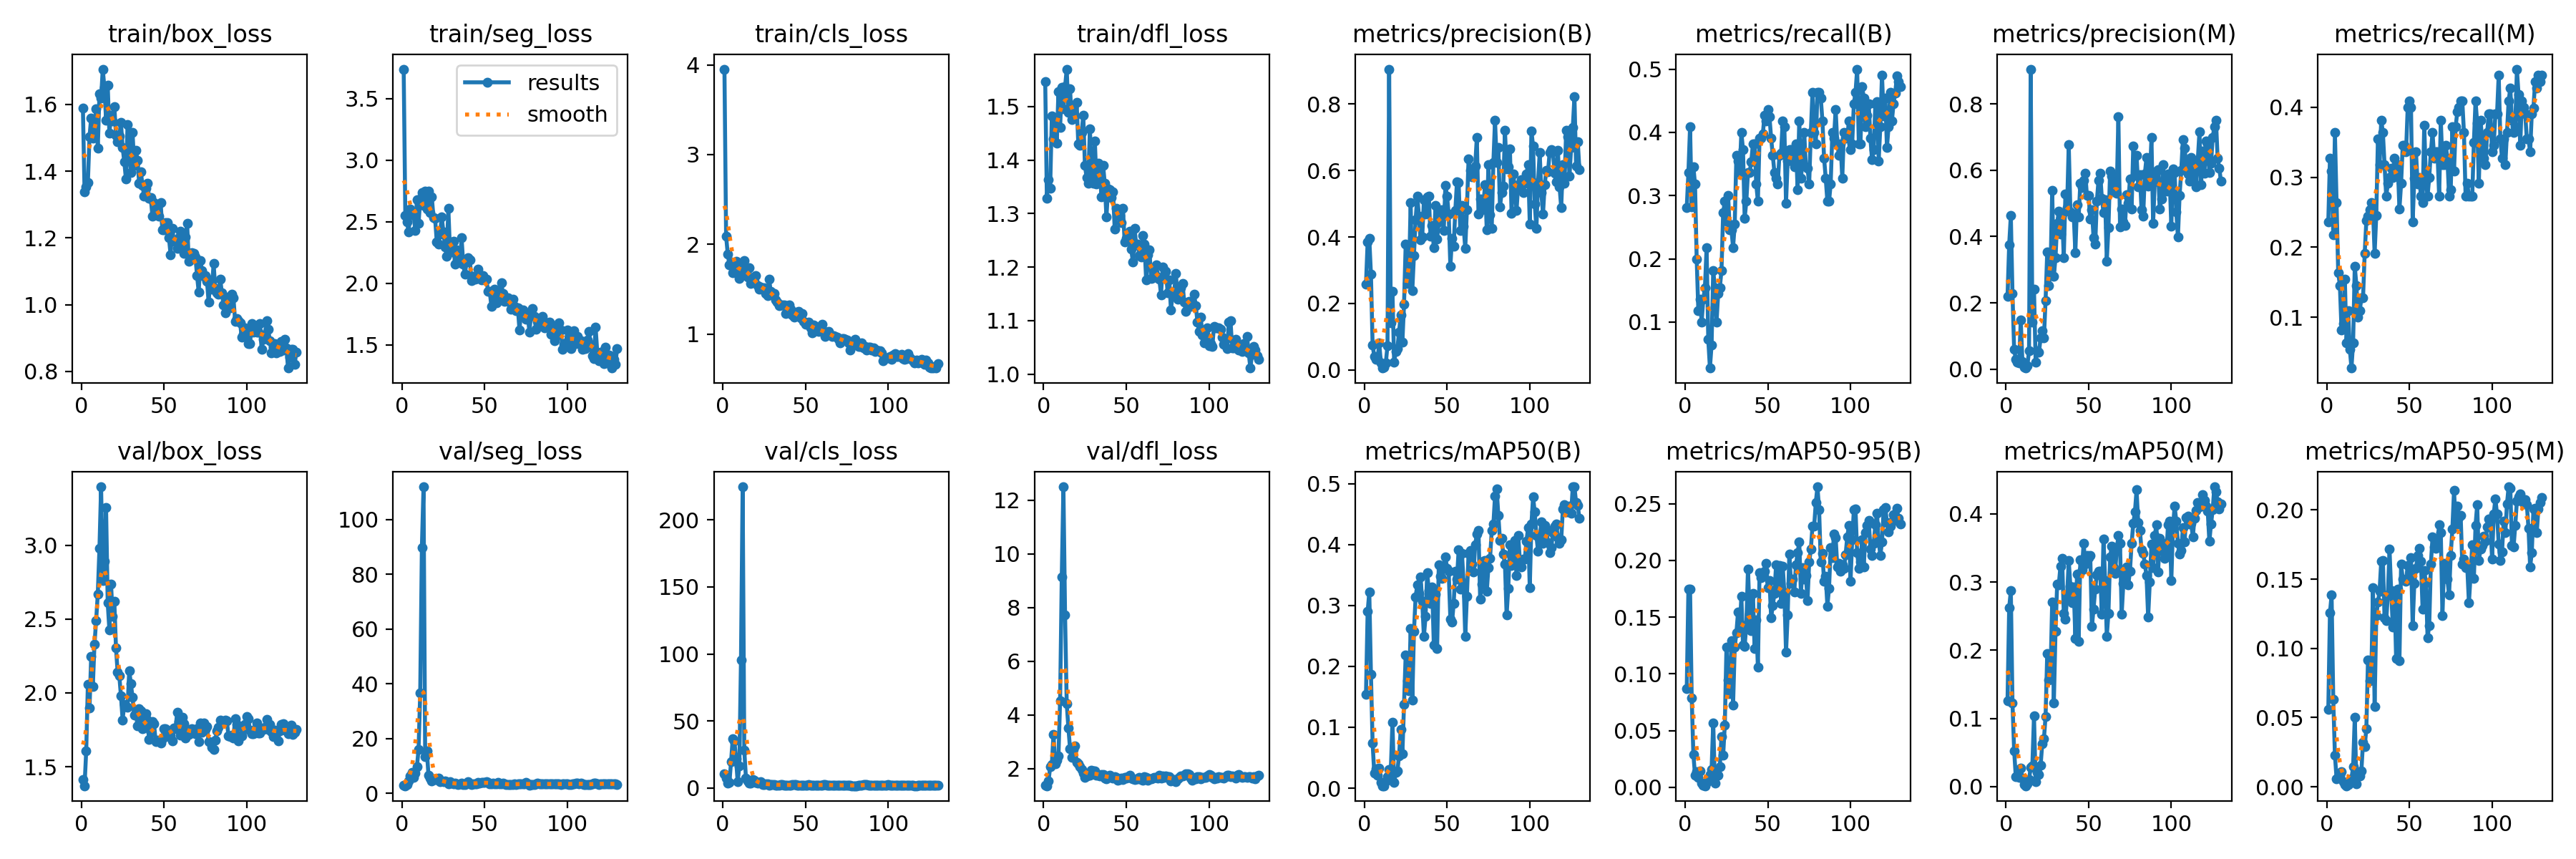
\includegraphics[scale=0.37]{Figures/segment/SegmentResults.png}
		\caption{YOLOv8s-Segment Results}
		\label{fig:YOLOv8s-Segment-Results}
	\end{figure}
	\subsubsection{YOLOv8n-Detect}
	
	\section{模型的评价与推广}
	\subsection{模型的评价}
	\begin{itemize}
		\item \textbf{模型的优点}

		\item \textbf{模型的缺点}

		\item \textbf{模型的改进}

	\end{itemize}
	\subsection{模型的推广}
	此模型具备分析及处理有明显特征的复杂图像的能力,因此除了估算坑洼占比,为道路避障和道路修复等工作提供便利外,我们也可以将其应用于人工智能驾驶的智能避障层面,以提供给乘客更加舒适的乘坐体验,同时也减少了坑洼可能对车辆造成的损坏,降低企业的车辆维护成本。以此类推,除了人工智能驾驶层面,此模型还可应用于环境保护,通过对坑洼面积占比的估算,帮助相关专家及工作人员了解地形地貌对于生态环境的影响,为环境保护工作提供一定的数据支持。

	\newpage
	
	\phantomsection
	\addcontentsline{toc}{section}{\textbf{参考文献}}
	\begin{spacing}{1.08}
	\begin{thebibliography}{99}
	\bibitem{YOLO任务}知乎.用YOLOv8一站式解决图像分类、检测、分割[EB/OL].\url{https://zhuanlan.zhihu.com/p/655889189}.

	\bibitem{YOLO架构}MMYOLO.Algorithm principles and implementation with YOLOv8 — MMYOLO 0.6.0 documentation[EB/OL].\url{https://mmyolo.readthedocs.io/en/latest/recommended_topics/algorithm_descriptions/yolov8_description.html}.

	\bibitem{YOLOv8简述}刘瑞锦,何章鸣.基于YOLOv8的卫星遥感图像快速目标检测方法[J].空间控制技术与应用,2023,49(05):89-97.

	\bibitem{YOLO数据增强}Zhang H, Cisse M, Dauphin Y N, et al. mixup: Beyond empirical risk minimization[J]. arXiv preprint arXiv:1710.09412, 2017.

	\bibitem{曹江华}曹江华. 复杂背景下非结构化道路可行驶区域检测研究[D].浙江科技学院,2021.

	\bibitem{Head}Song G, Liu Y, Wang X. Revisiting the sibling head in object detector[C]//Proceedings of the IEEE/CVF conference on computer vision and pattern recognition. 2020: 11563-11572.

	\bibitem{ISAT-SAM}Github.yatengLG/ISAT\_with\_segment\_anything: Labeling tool by SAM(segment anything model),supports SAM, sam-hq, MobileSAM etc.交互式半自动图像标注工具[EB/OL].\url{https://github.com/yatengLG/ISAT_with_segment_anything}.

	\bibitem{Labelimg}知乎.【教程】标注工具Labelimg的安装与使用[EB/OL].\url{https://zhuanlan.zhihu.com/p/550021453}.

	\bibitem{LOSS}CSDN.YOLO目标检测中损失函数loss的理解及部分代码实现[EB/OL].\url{https://blog.csdn.net/shengyan5515/article/details/84036734}.

	\bibitem{模型评测}知乎.模型评测:PRECISION、RECALL、F1-score[EB/OL].\url{https://zhuanlan.zhihu.com/p/519982682}.


	\bibitem{Yellowbrick}Yellowbrick.Precision-Recall Curves - Yellowbrick v1.5 documentation[EB/OL].\url{https://www.scikit-yb.org/en/latest/api/classifier/prcurve.html}.

	\bibitem{指标}CSDN.目标检测评估指标mAP:从Precision,Recall,到AP50-95【未完待续】[EB/OL].\url{https://blog.csdn.net/Albert233333/article/details/132752216}.

	\end{thebibliography}
	\end{spacing}
	\newpage

	\phantomsection
	\addcontentsline{toc}{section}{\textbf{附\hspace{2pc}录}}

	% \appendix
	% \ctexset{section={format={\zihao{-4}\heiti\raggedright}}}
	\begin{center}
		\heiti\zihao{4} 附\hspace{2pc}录
	\end{center}

% \phantomsection
% \addcontentsline{toc}{subsection}{[A]图示}
% 	% \section*{[A]图表}
% 	\noindent{\heiti [A]图示}
% \newpage
% \phantomsection
% \addcontentsline{toc}{subsection}{[B]支撑文件列表}
% 	% \section*{[B]支撑文件列表}
	\noindent{\heiti [A]支撑文件列表}
	~\\

	支撑文件列表如下(列表中不包含原始数据集):
	% Table generated by Excel2LaTeX from sheet 'Sheet2'
	\begin{table}[H]
		\centering
		\scalebox{0.9}{
		  \begin{tabular}{cc}
		  \toprule
		  \textbf{文件(夹)名} & \textbf{描述} \\
		  \midrule
		  html & 包括所有解决问题的源程序运行结果 \\
		  ipynb & 包括所有解决问题的源程序源代码 \\
		  models  & 已训练好的模型文件 \\
		  process & 包括所有模型训练、预测的过程结果 \\
		  py  & 包括所有解决问题的源程序输出python文件 \\
		  yaml & 包括所有模型训练的配置文件 \\
		  test\_result2.csv  & 坑洼面积占比估算结果 \\
		  \bottomrule
		  \end{tabular}}
	\end{table}
  
\newpage
% \phantomsection
% \addcontentsline{toc}{subsection}{[C]使用的软件、环境}
	% \section*{[C]使用的软件、环境}
	\noindent{\heiti [B]使用的软件、环境}
	% ~\\

	\textbf{B.1 使用的软件及版本}
	\begin{itemize}
		\item TeX Live 2022
		\item Visual Studio Code 1.85.0
		\item WPS Office 2023冬季更新(15990)
		\item Python 3.10.4 [MSC v.1929 64 bit (AMD64)] on win32
		\item Pycharm 2023.3 (Professional Edition)
	\end{itemize}
	
	\textbf{B.2 模型训练所用计算机配置}
	\begin{itemize}
		\item Intel(R) Core(TM) i5-10200H CPU @ 2.40GHz
		\item NVIDIA GeForce GTX 1650 Ti
		\item NVIDIA CUDA 11.7.102 driver
		\item 16.0 GB RAM
		\item Windows 10 家庭中文版 22H2
	\end{itemize}

	\textbf{B.3 Python环境下所用使用到的库及其版本}
\begin{table}[htbp]
	\centering
	\setlength{\aboverulesep}{0pt}
	\setlength{\belowrulesep}{0pt}
	\scalebox{0.9}{
	  \begin{tabular}{cc||cc}
	  \toprule
	  \textbf{库}     & \textbf{版本}    & \textbf{库}     & \textbf{版本} \\
	  \midrule
	  collections & 内置库   & jupyterlab-widgets & 3.0.9 \\
	  opencv-python & 4.8.1.78 & keras & 2.14.0 \\
	  h5py  & 3.10.0 & matplotlib & 3.8.0 \\
	  jupyter & 1.0.0 & numpy & 1.26.1 \\
	  jupyter\_client & 8.5.0 & os    & 内置库 \\
	  jupyter-console & 6.6.3 & pandas & 2.1.2 \\
	  jupyter\_core & 5.4.0 & pickle & 内置库 \\
	  jupyter-events & 0.8.0 & random & 内置库 \\
	  jupyter-lsp & 2.2.0 & shutil & 内置库 \\
	  jupyter\_server & 2.9.1 & sklearn & 1.3.2 \\
	  jupyter\_server\_terminals & 0.4.4 & tensorflow & 2.14.0 \\
	  jupyterlab & 4.0.7 & warnings & 内置库 \\
	  jupyterlab-pygments & 0.2.2 & yellowbrick & 1.50  \\
	  jupyterlab\_server & 2.25.0 &       &  \\
	  \bottomrule
	  \end{tabular}}
\end{table}

\newpage
% \phantomsection
% \addcontentsline{toc}{subsection}{[D]问题解决源程序}
	% \section*{[D]问题解决源程序}
\noindent{\heiti [C]问题解决源程序}

\textbf{C.1 Comparative Analysis of Normal and Potholes [正常与坑洼道路比较分析]}
\begin{python}
#!/usr/bin/env python
# coding: utf-8

# In[1]:


import cv2
import numpy as np
import matplotlib.pyplot as plt

# In[2]:


normalImg = cv2.imread('DATA\\normal\\normal133.jpg')
potholesImg = cv2.imread('DATA\\potholes\\potholes1.jpg')

# In[3]:


plt.rcParams['font.sans-serif'] = ['Times New Roman']
plt.rcParams['axes.unicode_minus'] = False


# In[4]:


def cv_show(img):
    b, g, r = cv2.split(img)
    img = cv2.merge([r, g, b])
    plt.imshow(img)


# In[5]:


cv_show(normalImg)

# In[6]:


cv_show(potholesImg)

# In[7]:


color = ('b', 'g', 'r')

for i, col in enumerate(color):
    histr = cv2.calcHist([normalImg], [i], None, [256], [0, 256])
    plt.plot(histr, color=col)

plt.legend(['Blue', 'Green', 'Red'])
plt.xlim([0, 256])
plt.xticks(fontsize=10)
plt.yticks(fontsize=10)
plt.title('(a) normal133.jpg', y=-0.2, fontsize=12)
plt.xlabel('Pixel Value', fontsize=11)
plt.ylabel('Number of Pixels', fontsize=11)
plt.savefig('Figures\\normal133RGB直方图.pdf', bbox_inches='tight')

# In[8]:


color = ('b', 'g', 'r')

for i, col in enumerate(color):
    histr = cv2.calcHist([potholesImg], [i], None, [256], [0, 256])
    plt.plot(histr, color=col)

plt.legend(['Blue', 'Green', 'Red'])
plt.xlim([0, 256])
plt.xticks(fontsize=10)
plt.yticks(fontsize=10)
plt.title('(b) potholes1.jpg', y=-0.2, fontsize=12)
plt.xlabel('Pixel Value', fontsize=11)
plt.ylabel('Number of Pixels', fontsize=11)
plt.savefig('Figures\\potholes1RGB直方图.pdf', bbox_inches='tight')

# In[9]:


plt.style.use('ggplot')
plt.hist(normalImg.ravel(), 256, [0, 256], color='grey')
plt.title('(a) normal133.jpg', y=-0.2, fontsize=12)
plt.xlabel('Pixel Value', fontsize=11)
plt.ylabel('Number of Pixels', fontsize=11)
plt.savefig('Figures\\normal133灰度直方图.pdf', bbox_inches='tight')

# In[10]:


plt.style.use('ggplot')
plt.hist(potholesImg.ravel(), 256, [0, 256], color='grey')
plt.title('(b) potholes1.jpg', y=-0.2, fontsize=12)
plt.xlabel('Pixel Value', fontsize=11)
plt.ylabel('Number of Pixels', fontsize=11)
plt.savefig('Figures\\potholes1灰度直方图.pdf', bbox_inches='tight')

# In[11]:


# 边缘检测
gray = cv2.cvtColor(normalImg, cv2.COLOR_BGR2GRAY)
edges = cv2.Canny(gray, 100, 200)
plt.imshow(edges, cmap='gray')
plt.title('(a) normal133.jpg', y=-0.2, fontsize=12)
plt.savefig('Figures\\normal133边缘检测.pdf', bbox_inches='tight')

# In[12]:


# 边缘检测
gray = cv2.cvtColor(potholesImg, cv2.COLOR_BGR2GRAY)
edges = cv2.Canny(gray, 100, 200)
plt.imshow(edges, cmap='gray')
plt.title('(b) potholes1.jpg', y=-0.2, fontsize=12)
plt.savefig('Figures\\potholes1边缘检测.pdf', bbox_inches='tight')

# In[13]:


plt.imshow(normalImg)
plt.colorbar()
plt.title('(a) normal133.jpg', y=-0.3, fontsize=12)
plt.savefig('Figures\\normal133热力图.pdf')

# In[14]:


plt.imshow(potholesImg)
plt.colorbar()
plt.title('(b) potholes1.jpg', y=-0.3, fontsize=12)
plt.savefig('Figures\\potholes1热力图.pdf')

# In[15]:


# 阈值分割
hsv = cv2.cvtColor(normalImg, cv2.COLOR_BGR2HSV)
lower_blue = np.array([90, 50, 50])
upper_blue = np.array([130, 255, 255])
mask = cv2.inRange(hsv, lower_blue, upper_blue)
plt.imshow(mask, cmap='gray')
plt.title('(a) normal133.jpg', y=-0.2, fontsize=12)
plt.savefig('Figures\\normal133阈值分割.pdf', bbox_inches='tight')

# In[16]:


# 阈值分割
hsv = cv2.cvtColor(potholesImg, cv2.COLOR_BGR2HSV)
lower_blue = np.array([90, 50, 50])
upper_blue = np.array([130, 255, 255])
mask = cv2.inRange(hsv, lower_blue, upper_blue)
plt.imshow(mask, cmap='gray')
plt.title('(b) potholes1.jpg', y=-0.2, fontsize=12)
plt.savefig('Figures\\potholes1阈值分割.pdf', bbox_inches='tight')

# In[17]:


# 转换为灰度图像
gray = cv2.cvtColor(normalImg, cv2.COLOR_BGR2GRAY)
# 二值化
ret, binary = cv2.threshold(gray, 0, 255, cv2.THRESH_BINARY | cv2.THRESH_OTSU)
# 轮廓检测
contours, hierarchy = cv2.findContours(binary, cv2.RETR_TREE, cv2.CHAIN_APPROX_SIMPLE)
# 绘制轮廓
cv2.drawContours(normalImg, contours, -1, (0, 0, 255), 3)

plt.subplot(1, 2, 1)
plt.title('(a) Original', y=-0.4, fontsize=12)
plt.imshow(normalImg)
plt.subplot(1, 2, 2)
plt.imshow(binary, cmap='gray')
plt.title('(b) Contours', y=-0.4, fontsize=12)
plt.savefig('Figures\\normal133轮廓检测.pdf', bbox_inches='tight')

# In[18]:


# 转换为灰度图像
gray = cv2.cvtColor(potholesImg, cv2.COLOR_BGR2GRAY)
# 二值化
ret, binary = cv2.threshold(gray, 0, 255, cv2.THRESH_BINARY | cv2.THRESH_OTSU)
# 轮廓检测
contours, hierarchy = cv2.findContours(binary, cv2.RETR_TREE, cv2.CHAIN_APPROX_SIMPLE)
# 绘制轮廓
cv2.drawContours(potholesImg, contours, -1, (0, 0, 255), 3)

plt.subplot(1, 2, 1)
plt.title('(a) Original', y=-0.4, fontsize=12)
plt.imshow(potholesImg)
plt.subplot(1, 2, 2)
plt.imshow(binary, cmap='gray')
plt.title('(b) Contours', y=-0.4, fontsize=12)
plt.savefig('Figures\\potholes1轮廓检测.pdf', bbox_inches='tight')
\end{python}

\textbf{C.2 Data Preprocessing [数据预处理]}
\begin{python}
#!/usr/bin/env python
# coding: utf-8

# In[1]:


import os
import shutil

# 指定目录"DATA"
path = "DATA"

# 在"DATA"文件夹中创建"normal"和"potholes"文件夹
os.mkdir(os.path.join(path, "normal"))
os.mkdir(os.path.join(path, "potholes"))

# 读取"DATA"文件夹,若文件名中含有"normal",则将其放置于"normal"文件夹中,否则放置于"potholes"文件夹中
files = os.listdir(path)
for file in files:
    if "normal" in file:
        shutil.move(os.path.join(path, file), os.path.join(path, "normal"))
    else:
        shutil.move(os.path.join(path, file), os.path.join(path, "potholes"))

\end{python}

\textbf{C.3 Images Display [图像展示]}
\begin{python}
#!/usr/bin/env python
# coding: utf-8

# In[1]:


import cv2

img = cv2.imread("DATA\\potholes\\potholes1.jpg", cv2.IMREAD_COLOR)
img = cv2.resize(img, [256, 256])

Gaussian = cv2.GaussianBlur(img, (3, 3), 1)
Bilateral = cv2.bilateralFilter(img, 9, 75, 75)
Rotate = cv2.warpAffine(img, cv2.getRotationMatrix2D((img.shape[1] / 2, img.shape[0] / 2), 30, 1),
                        (img.shape[1], img.shape[0]))

cv2.imwrite("potholes1_Gaussian.jpg", Gaussian)
cv2.imwrite("potholes1_Bilateral.jpg", Bilateral)
cv2.imwrite("potholes1_Rotate.jpg", Rotate)

\end{python}

\textbf{C.4 isat2txt [isat转txt]}
\begin{python}
import json
import os
import shutil

category_mapping = {"potholes": 0}
# ISAT格式的实例分割标注文件
ISAT_FOLDER = "./annotations"
# YOLO格式的实例分割标注文件
YOLO_FOLDER = "./labels"

# 创建YoloV8标注的文件夹
if not os.path.exists(YOLO_FOLDER):
    os.makedirs(YOLO_FOLDER)


# 载入所有的ISAT的JSON文件
for filename in os.listdir(ISAT_FOLDER):
    if not filename.endswith(".json"):
        # 不是json格式, 跳过
        continue
    # 载入ISAT的JSON文件
    with open(os.path.join(ISAT_FOLDER, filename), "r") as f:
        isat = json.load(f)
    # 提取文件名(不带文件后缀)
    image_name = filename.split(".")[0]
    # Yolo格式的标注文件名, 后缀是txt
    yolo_filename = f"{image_name}.txt"
    # 写入信息
    with open(os.path.join(YOLO_FOLDER, yolo_filename), "w") as f:
        # 获取图像信息
        # - 图像宽度

        image_width = isat["info"]["width"]

        # try:
        #     image_width = isat["info"]["width"]
        # except KeyError:
        #     break
        # - 图像高度
        image_height = isat["info"]["height"]
        # 获取实例标注数据
        for annotation in isat["objects"]:
            # 获取类别名称
            category_name = annotation["category"]
            # 如果不在类别名称字典里面,跳过
            if category_name not in category_mapping:
                continue
            # 从字典里面查询类别ID
            category_id = category_mapping[category_name]
            # 提取分割信息
            segmentation = annotation["segmentation"]
            segmentation_yolo = []
            # 遍历所有的轮廓点
            for segment in segmentation:
                # 提取轮廓点的像素坐标 x, y
                x, y = segment
                # 归一化处理
                x_center = x/image_width
                y_center = y/image_height
                # 添加到segmentation_yolo里面
                segmentation_yolo.append(f"{x_center:.4f} {y_center:.4f}")
            segmentation_yolo_str = " ".join(segmentation_yolo)
            # 添加一行Yolo格式的实例分割数据
            # 格式如下: class_id x1 y1 x2 y2 ... xn yn\n
            f.write(f"{category_id} {segmentation_yolo_str}\n")
\end{python}

\textbf{C.5 xml2txt [xml转txt]}
\begin{python}
import xml.etree.ElementTree as ET
import os, cv2
import numpy as np
from os import listdir
from os.path import join

#将给定的XML格式的标注文件转换为YOLOv8所需的TXT格式,并记录数据集中的类别信息
classes = []

def convert(size, box):
    dw = 1. / (size[0])
    dh = 1. / (size[1])
    x = (box[0] + box[1]) / 2.0 - 1
    y = (box[2] + box[3]) / 2.0 - 1
    w = box[1] - box[0]
    h = box[3] - box[2]
    x = x * dw
    w = w * dw
    y = y * dh
    h = h * dh
    return (x, y, w, h)


def convert_annotation(xmlpath, xmlname):
    with open(xmlpath, "r", encoding='utf-8') as in_file:
        txtname = xmlname[:-4] + '.txt'
        txtfile = os.path.join(txtpath, txtname)
        tree = ET.parse(in_file)
        root = tree.getroot()
        filename = root.find('filename')
        img = cv2.imdecode(np.fromfile('{}/{}.{}'.format(imgpath, xmlname[:-4], postfix), np.uint8), cv2.IMREAD_COLOR)
        h, w = img.shape[:2]
        res = []
        for obj in root.iter('object'):
            cls = obj.find('name').text
            if cls not in classes:
                classes.append(cls)
            cls_id = classes.index(cls)
            xmlbox = obj.find('bndbox')
            b = (float(xmlbox.find('xmin').text), float(xmlbox.find('xmax').text), float(xmlbox.find('ymin').text),
                 float(xmlbox.find('ymax').text))
            bb = convert((w, h), b)
            res.append(str(cls_id) + " " + " ".join([str(a) for a in bb]))
        if len(res) != 0:
            with open(txtfile, 'w+') as f:
                f.write('\n'.join(res))


if __name__ == "__main__":
    postfix = 'jpg'
    imgpath = 'VOCdevkit/JPEGImages'
    xmlpath = 'VOCdevkit/Annotations'
    txtpath = 'VOCdevkit/txt'
    
    if not os.path.exists(txtpath):
        os.makedirs(txtpath, exist_ok=True)
    
    list = os.listdir(xmlpath)
    error_file_list = []
    for i in range(0, len(list)):
        try:
            path = os.path.join(xmlpath, list[i])
            if ('.xml' in path) or ('.XML' in path):
                convert_annotation(path, list[i])
                print(f'file {list[i]} convert success.')
            else:
                print(f'file {list[i]} is not xml format.')
        except Exception as e:
            print(f'file {list[i]} convert error.')
            print(f'error message:\n{e}')
            error_file_list.append(list[i])
    print(f'this file convert failure\n{error_file_list}')
    print(f'Dataset Classes:{classes}')
\end{python}

\textbf{C.6 Segment Spilt Data [图像分割数据集划分]}
\begin{python}
import os
import random
from tqdm import tqdm

# 指定 images 文件夹路径
image_dir = "./images"
# 指定 labels 文件夹路径
label_dir = "./labels"
# 创建一个空列表来存储有效图片的路径
valid_images = []
# 创建一个空列表来存储有效 label 的路径
valid_labels = []

# 遍历 images 文件夹下的所有图片
for image_name in os.listdir(image_dir):
    # 获取图片的完整路径
    image_path = os.path.join(image_dir, image_name)
    # 获取图片文件的扩展名
    ext = os.path.splitext(image_name)[-1]
    # 根据扩展名替换成对应的 label 文件名
    label_name = image_name.replace(ext, ".txt")
    # 获取对应 label 的完整路径
    label_path = os.path.join(label_dir, label_name)
    # 判断 label 是否存在
    if not os.path.exists(label_path):
        # 删除图片
        os.remove(image_path)
        print("deleted:", image_path)
    else:
        # 将图片路径添加到列表中
        valid_images.append(image_path)
        # 将label路径添加到列表中
        valid_labels.append(label_path)
        # print("valid:", image_path, label_path)
# 遍历每个有效图片路径
for i in tqdm(range(len(valid_images))):
    image_path = valid_images[i]
    label_path = valid_labels[i]
    # 随机生成一个概率
    r = random.random()
    # 判断图片应该移动到哪个文件夹
    # train:valid:test = 7:2:1
    if r < 0.1:
        # 移动到 test 文件夹
        destination = "./datasets/test"
    elif r < 0.3:
        # 移动到 valid 文件夹
        destination = "./datasets/valid"
    else:
        # 移动到 train 文件夹
        destination = "./datasets/train"
    # 生成目标文件夹中图片的新路径
    image_destination_path = os.path.join(destination, "images", os.path.basename(image_path))
    # 移动图片到目标文件夹
    os.rename(image_path, image_destination_path)
    # 生成目标文件夹中 label 的新路径
    label_destination_path = os.path.join(destination, "labels", os.path.basename(label_path))
    # 移动 label 到目标文件夹
    os.rename(label_path, label_destination_path)
print("valid images:", valid_images)
# 输出有效label路径列表
print("valid labels:", valid_labels)
\end{python}

\textbf{C.7 Detect Spilt Data [图像检测数据集划分]}
\begin{python}
import os, shutil
from sklearn.model_selection import train_test_split

# 用于将图像和标注文件按照一定比例划分为训练集、验证集和测试集,并将它们分别复制到相应的文件夹中
val_size = 0.1
test_size = 0.1
postfix = 'jpg'
imgpath = 'VOCdevkit/JPEGImages'
txtpath = 'VOCdevkit/txt'

os.makedirs('images/train', exist_ok=True)
os.makedirs('images/val', exist_ok=True)
os.makedirs('images/test', exist_ok=True)
os.makedirs('labels/train', exist_ok=True)
os.makedirs('labels/val', exist_ok=True)
os.makedirs('labels/test', exist_ok=True)

listdir = [i for i in os.listdir(txtpath) if 'txt' in i]
train, test = train_test_split(listdir, test_size=test_size, shuffle=True, random_state=0)
train, val = train_test_split(train, test_size=val_size, shuffle=True, random_state=0)
print(f'train set size:{len(train)} val set size:{len(val)} test set size:{len(test)}')

for i in train:
    shutil.copy('{}/{}.{}'.format(imgpath, i[:-4], postfix), 'images/train/{}.{}'.format(i[:-4], postfix))
    shutil.copy('{}/{}'.format(txtpath, i), 'labels/train/{}'.format(i))

for i in val:
    shutil.copy('{}/{}.{}'.format(imgpath, i[:-4], postfix), 'images/val/{}.{}'.format(i[:-4], postfix))
    shutil.copy('{}/{}'.format(txtpath, i), 'labels/val/{}'.format(i))

for i in test:
    shutil.copy('{}/{}.{}'.format(imgpath, i[:-4], postfix), 'images/test/{}.{}'.format(i[:-4], postfix))
    shutil.copy('{}/{}'.format(txtpath, i), 'labels/test/{}'.format(i))
\end{python}

\textbf{C.8 YOLOv8s Segment [YOLOv8s图像分割]}
\begin{python}
#!/usr/bin/env python
# coding: utf-8

# In[1]:


from ultralytics import YOLO

# In[3]:


model = YOLO('yolov8s-seg.pt')
results = model.train(data="dataset/VOCdevkit/datasets/potholes.yaml", epochs=300, device='cpu')

# In[2]:


model = YOLO('potholesSegment.pt')

# In[3]:


resultOne = model('potholes\\part1', save=True)

# In[4]:


resultTwo = model('potholes\\part2', save=True)

# In[5]:


resultThree = model('potholes\\part3', save=True)

# In[3]:


resultFour = model('potholes\\part4', save=True)

# In[4]:


resultFive = model('potholes\\part5', save=True)

# In[3]:


resultSix = model('potholes\\part6', save=True)

# In[4]:


resultSeven = model('potholes\\part7', save=True)

# In[3]:


resultEight = model('potholes\\part8', save=True)
\end{python}

\textbf{C.9 YOLOv8n Detect [YOLOv8n图像检测]}
\begin{python}
#!/usr/bin/env python
# coding: utf-8

# In[1]:


from ultralytics import YOLO


# In[47]:


model = YOLO("potholesDetect.pt")
resultsOne = model.predict(source="potholes\\partOne", save=True, save_conf=True, save_txt=True,imgsz=416)


# In[48]:


model = YOLO("potholesDetect.pt")
resultsTwo = model.predict(source="potholes\\partTwo", save=True, save_conf=True, save_txt=True,imgsz=416)
\end{python}

\textbf{C.10 Coordinate Transformation [坐标转换]}
\begin{python}
#!/usr/bin/env python
# coding: utf-8

# In[1]:


import os
import cv2
import torch
import numpy as np

# In[2]:


label_path = 'potholes\labels'
image_path = 'potholes\images'


def xywhn2xyxy(x, w=416, h=416, padw=0, padh=0):
    y = x.clone() if isinstance(x, torch.Tensor) else np.copy(x)
    y[:, 0] = w * (x[:, 0] - x[:, 2] / 2) + padw  # top left x
    y[:, 1] = h * (x[:, 1] - x[:, 3] / 2) + padh  # top left y
    y[:, 2] = w * (x[:, 0] + x[:, 2] / 2) + padw  # bottom right x
    y[:, 3] = h * (x[:, 1] + x[:, 3] / 2) + padh  # bottom right y
    return y


folder = os.path.exists('potholes\\labelsNew')
if not folder:
    os.makedirs('potholes\\labelsNew')

folderlist = os.listdir(label_path)
for i in folderlist:
    label_path_new = os.path.join(label_path, i)
    with open(label_path_new, 'r') as f:
        lb = np.array([x.split() for x in f.read().strip().splitlines()], dtype=np.float32)  # labels
        print(lb)
    read_label = label_path_new.replace(".txt", ".jpg")
    read_label_path = read_label.replace(label_path, image_path)
    print(read_label_path, "ddd")
    img = cv2.imread(str(read_label_path))
    h, w = img.shape[:2]
    lb[:, 1:] = xywhn2xyxy(lb[:, 1:], w, h, 0, 0)

    for _, x in enumerate(lb):
        class_label = int(x[0])

        with open('potholes\\labelsNew\\' + i, 'a') as fw:
            fw.write(str(int(x[0])) + ' ' + str(x[5]) + ' ' + str(x[1]) + ' ' + str(x[2]) + ' ' + str(x[3]) + ' ' + str(
                x[4]) + '\n')
\end{python}

\textbf{C.11 Proportional Calculation [面积占比估算]}
\begin{python}
#!/usr/bin/env python
# coding: utf-8

# In[1]:


import os
import cv2
import numpy as np
import pandas as pd

# In[2]:


labelsList = os.listdir('potholes\\labelsNew')
imagesList = os.listdir('potholes\\images')

# In[3]:


labelsDf = pd.DataFrame(labelsList, columns=['fnames'])
labelsDf

# In[4]:


Npotholes = pd.read_csv('potholes\\detectResults.txt', sep=' ', header=None)
Npotholes = Npotholes.drop([0, 1, 3, 5, 6], axis=1)
Npotholes.columns = ['fnames', 'Npotholes']
Npotholes['fnames'] = Npotholes['fnames'].str.split('\\').str[-1]
Npotholes['Npotholes'] = Npotholes['Npotholes'].str.replace('(', '')
Npotholes['fnames'] = Npotholes['fnames'].str.replace(':', '')
Npotholes

# In[5]:


Npotholes['Npotholes'] = Npotholes['Npotholes'].str.replace('no', '0')
Npotholes['Npotholes'] = Npotholes['Npotholes'].astype('int')
Npotholes

# In[6]:


data = pd.DataFrame(columns=['Type', '置信度', 'x1', 'y1', 'x2', 'y2', 'fnames'])
data

# In[7]:


for i in labelsList:
    with open('potholes\\labelsNew\\' + i, 'r') as f:
        content = f.readlines()
        lb = np.array([x.strip().split() for x in content], dtype=np.float32)  # labels
        lb = pd.DataFrame(lb, columns=['Type', '置信度', 'x1', 'y1', 'x2', 'y2'])
        lb['fnames'] = i

    data = data._append(lb, ignore_index=True)

data

# In[8]:


data = data.drop('Type', axis=1)
data = data[['fnames', '置信度', 'x1', 'y1', 'x2', 'y2']]
data['fnames'] = data['fnames'].str.replace('.txt', '.jpg')
data

# In[9]:


data = pd.merge(data, Npotholes, on='fnames', how='right')
data

# In[10]:


potholesImages = pd.DataFrame(imagesList, columns=['fnames'])
potholesImages

# In[11]:


for i in imagesList:
    img = cv2.imread('potholes\\images\\' + i)
    height, width, channels = img.shape
    potholesImages.loc[potholesImages['fnames'] == i, 'height'] = height
    potholesImages.loc[potholesImages['fnames'] == i, 'width'] = width

potholesImages

# In[12]:


data = pd.merge(data, potholesImages, on='fnames', how='left')
data

# In[13]:


data['S'] = data['height'] * data['width']
data['X'] = data['x2'] - data['x1']
data['Y'] = data['y2'] - data['y1']
data['Spotholes'] = data['X'] * data['Y']
data['Spotholes/S'] = data['Spotholes'] / data['S'] * 100
data

# In[14]:


data['Spotholes/S'] = data['Spotholes/S'].fillna(data['Spotholes/S'].mean())
data['Spotholes/S'] = data['Spotholes/S'].apply(np.ceil)
data['Spotholes/S'] = data['Spotholes/S'].astype('int')
data

# In[15]:


dataNew = data.groupby('fnames').apply(lambda x: x.loc[x['Spotholes/S'].idxmax()])
dataNew

# In[16]:


dataNew = dataNew.reset_index(drop=True)
dataNew

# In[17]:


dataR = pd.read_csv('未知数据集预测效果.csv')
dataR = dataR.drop(['imgType', 'label', 'isTrue'], axis=1)
dataR

# In[18]:


Results = pd.merge(dataR, dataNew, on='fnames', how='left')
Results

# In[19]:


# 修改guy7iodk.jpg行,height=1587,width=1200,S=1587*1200=1904400,Spotholes=954792,Spotholes/S=50
Results.loc[Results['fnames'] == 'guy7iodk.jpg', 'height'] = 1587
Results.loc[Results['fnames'] == 'guy7iodk.jpg', 'width'] = 1200
Results.loc[Results['fnames'] == 'guy7iodk.jpg', 'S'] = 1904400
Results.loc[Results['fnames'] == 'guy7iodk.jpg', 'Spotholes'] = 954792
Results.loc[Results['fnames'] == 'guy7iodk.jpg', 'Spotholes/S'] = 50
Results

# In[20]:


Results.loc[Results['imgClass'] == 'normal', 'Spotholes/S'] = 0
Results

# In[21]:


Results['Spotholes/S'] = Results['Spotholes/S'].astype('int')
Results

# In[22]:


Results.to_csv('SpotholesS.csv', index=False)
\end{python}

\textbf{C.12 Detect Segment Analyze [图像检测与图像分割效果分析]}
\begin{python}
#!/usr/bin/env python
# coding: utf-8

# In[1]:


import pandas as pd

dataDetect = pd.read_csv('detectResults.txt', sep=' ', header=None)
dataSegment = pd.read_csv('segmentResults.txt', sep=' ', header=None)

# In[2]:


dataDetect = dataDetect.drop([0, 1, 3, 5, 6], axis=1)
dataDetect.columns = ['fnames', 'Detect-Npotholes']
dataDetect['fnames'] = dataDetect['fnames'].str.split('\\').str[-1]
dataDetect['Detect-Npotholes'] = dataDetect['Detect-Npotholes'].str.replace('(', '')
dataDetect['fnames'] = dataDetect['fnames'].str.replace(':', '')
dataDetect['Detect-Npotholes'] = dataDetect['Detect-Npotholes'].str.replace('no', '0')
dataDetect['Detect-Npotholes'] = dataDetect['Detect-Npotholes'].astype('int')
dataDetect

# In[3]:


dataSegment = dataSegment.drop([0, 1, 3, 5, 6], axis=1)
dataSegment.columns = ['fnames', 'Segment-Npotholes']
dataSegment['fnames'] = dataSegment['fnames'].str.split('\\').str[-1]
dataSegment['Segment-Npotholes'] = dataSegment['Segment-Npotholes'].str.replace('(', '')
dataSegment['fnames'] = dataSegment['fnames'].str.replace(':', '')
dataSegment['Segment-Npotholes'] = dataSegment['Segment-Npotholes'].str.replace('no', '0')
dataSegment['Segment-Npotholes'] = dataSegment['Segment-Npotholes'].astype('int')
dataSegment

# In[4]:


data = pd.merge(dataDetect, dataSegment, on='fnames', how='left')
data

# In[5]:


# DetectFalse为Detect-Npotholes为0的个数
# DetectTrue为Detect-Npotholes不为0的个数
# SegmentFalse为Segment-Npotholes为0的个数
# SegmentTrue为Segment-Npotholes不为0的个数
DetectFalse = 0
DetectTrue = 0
SegmentFalse = 0
SegmentTrue = 0
for i in range(len(data)):
    if data['Detect-Npotholes'][i] == 0:
        DetectFalse += 1
    else:
        DetectTrue += 1
    if data['Segment-Npotholes'][i] == 0:
        SegmentFalse += 1
    else:
        SegmentTrue += 1

# In[6]:


DetectTrue / (DetectFalse + DetectTrue)

# In[7]:


SegmentTrue / (SegmentFalse + SegmentTrue)
\end{python}

\newpage
% \phantomsection
% \addcontentsline{toc}{subsection}{[D]问题解决源程序}
	% \section*{[D]问题解决源程序}
\noindent{\heiti [D]模型训练配置文件}

\textbf{D.1 segment.yaml}
\begin{python}
# Train/val/test sets as 1) dir: path/to/imgs, 2) file: path/to/imgs.txt, or 3) list: [path/to/imgs1, path/to/imgs2, ..]
# path: ../datasets  # dataset root dir
train: E:/University/PythonProject/UltralyticsPotholes/dataset/VOCdevkit/datasets/train/images  # train images (relative to 'path') 128 images
val: E:/University/PythonProject/UltralyticsPotholes/dataset/VOCdevkit/datasets/valid/images  # val images (relative to 'path') 128 images
test: E:/University/PythonProject/UltralyticsPotholes/dataset/VOCdevkit/datasets/test/images # test images (optional)

# Classes
names:
  0: potholes
\end{python}

\textbf{D.2 detect.yaml}
\begin{python}
# dataset path
train: E:/University/PythonProject/UltralyticsMaster/dataset/images/train
val: E:/University/PythonProject/UltralyticsMaster/dataset/images/val
test: E:/University/PythonProject/UltralyticsMaster/dataset/images/test

# number of classes
nc: 1

# class names
names: ['potholes']
\end{python}

\textbf{D.3 YOLOv8-seg.yaml}
\begin{python}
# Parameters
nc: 1  # number of classes
scales: # model compound scaling constants, i.e. 'model=yolov8n-seg.yaml' will call yolov8-seg.yaml with scale 'n'
  # [depth, width, max_channels]
  n: [0.33, 0.25, 1024]
  s: [0.33, 0.50, 1024]
  m: [0.67, 0.75, 768]
  l: [1.00, 1.00, 512]
  x: [1.00, 1.25, 512]

# YOLOv8.0n backbone
backbone:
  # [from, repeats, module, args]
  - [-1, 1, Conv, [64, 3, 2]]  # 0-P1/2
  - [-1, 1, Conv, [128, 3, 2]]  # 1-P2/4
  - [-1, 3, C2f, [128, True]]
  - [-1, 1, Conv, [256, 3, 2]]  # 3-P3/8
  - [-1, 6, C2f, [256, True]]
  - [-1, 1, Conv, [512, 3, 2]]  # 5-P4/16
  - [-1, 6, C2f, [512, True]]
  - [-1, 1, Conv, [1024, 3, 2]]  # 7-P5/32
  - [-1, 3, C2f, [1024, True]]
  - [-1, 1, SPPF, [1024, 5]]  # 9

# YOLOv8.0n head
head:
  - [-1, 1, nn.Upsample, [None, 2, 'nearest']]
  - [[-1, 6], 1, Concat, [1]]  # cat backbone P4
  - [-1, 3, C2f, [512]]  # 12

  - [-1, 1, nn.Upsample, [None, 2, 'nearest']]
  - [[-1, 4], 1, Concat, [1]]  # cat backbone P3
  - [-1, 3, C2f, [256]]  # 15 (P3/8-small)

  - [-1, 1, Conv, [256, 3, 2]]
  - [[-1, 12], 1, Concat, [1]]  # cat head P4
  - [-1, 3, C2f, [512]]  # 18 (P4/16-medium)

  - [-1, 1, Conv, [512, 3, 2]]
  - [[-1, 9], 1, Concat, [1]]  # cat head P5
  - [-1, 3, C2f, [1024]]  # 21 (P5/32-large)

  - [[15, 18, 21], 1, Segment, [nc, 32, 256]]  # Segment(P3, P4, P5)
\end{python}

\newpage
% \phantomsection
% \addcontentsline{toc}{subsection}{[D]问题解决源程序}
	% \section*{[D]问题解决源程序}
\noindent{\heiti [D]图示}
\begin{figure}[H]
	\centering
	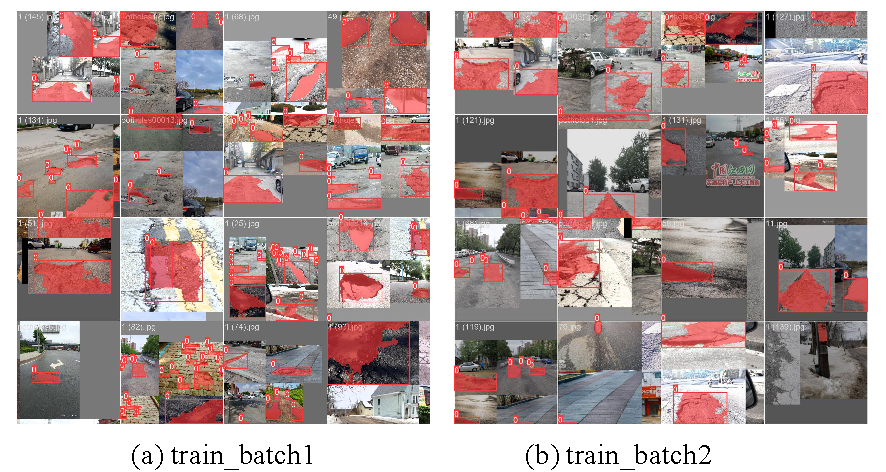
\includegraphics[width=0.8\textwidth]{Figures/segment/附Segment训练.pdf}
	\caption{附Segment训练}
	\label{fig:附Segment训练}
\end{figure}
\begin{figure}[H]
	\centering
	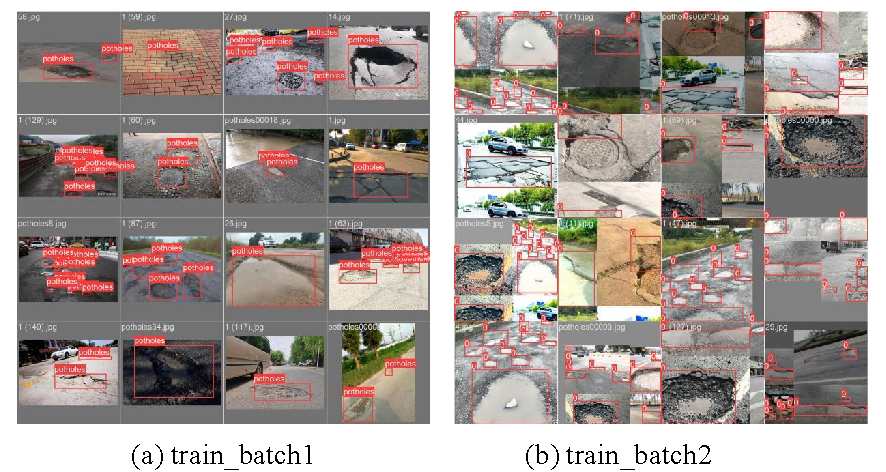
\includegraphics[width=0.8\textwidth]{Figures/detect/附Detect训练.pdf}
	\caption{附Detect训练}
	\label{fig:附Detect训练}
\end{figure}
\end{document}